\documentclass[12pt,a4paper]{report}
\usepackage{Bath-CS-Dissertation}
\usepackage[newfloat]{minted}
\usepackage[english]{babel}
\usepackage{amsthm}
\usepackage{amsmath}
\usepackage{stmaryrd}
\usepackage{amssymb}
\usemintedstyle{vs}
\usepackage{caption}
\usepackage{booktabs}
\usepackage{subcaption}

\title{SPCF: Interpreter Development and Affine Program Transformation Showcase}
\author{Jay Rabjohns}
\date{Bachelor of Science in Computer Science\\ 
      The University of Bath\\
      2023/2024}

% Numberings for Listing
\makeatletter
%\renewcommand*{\thelisting}{\thesection.\arabic{listing}}
\renewcommand*{\thelisting}{\thechapter.\arabic{listing}}
\@addtoreset{listing}{section}
\makeatother

% Numberings for theorems, corollaries, and lemmas
\newtheorem{theorem}{Theorem}[section]
\newtheorem{corollary}{Corollary}[theorem]
\newtheorem{lemma}[theorem]{Lemma}

\theoremstyle{definition}
\newtheorem{proposition}{Proposition}[chapter]

\theoremstyle{definition}
\newtheorem{definition}{Definition}[chapter]%section]

\theoremstyle{remark}
\newtheorem*{remark}{Remark}

\begin{document}
\hypersetup{pageanchor=false}

% Set this to the language you want to use in your code listings (if any)
\lstset{language=Haskell,breaklines,breakatwhitespace,basicstyle=\small}

\setcounter{page}{0}
\pagenumbering{roman}

\maketitle
\newpage

\declaration{SPCF: Interpreter Development and Affine Program Transformation Showcase}{Jay Rabjohns}
\newpage

\hypersetup{pageanchor=true}
\abstract

We explore the concept of function denesting in SPCF, a derivative of typed $\lambda$-calculus with non-local control. Function nesting involves sharing variables from one function’s scope with another function's arguments. This transformation is based on the work of Laird who provides denotational semantics for a retraction on terms of a higher type into a lower one, and can be seen as rewriting programs to adhere to affine typing rules. We illustrate this transformation working in the real world and evaluate its benefits. 

As part of the project we also build and release an interpreter for SPCF, a language that currently lacks one which is widely available. This both has the focus of illustrating the denesting action working, as well as contributing to the language’s ecosystem, hopefully making it easier to experiment with the language.
\newpage

\tableofcontents
\newpage

\listoffigures
\newpage

\listoftables
\newpage

%%%%%%%%%%%%%%%%%%%%%%%%%%%%%%%%%%%%%%%%%%%%%%%%%%%%%%%%%%%%%%%%%%%%%%%%%%%%%%%%
\chapter*{Acknowledgements}
Firstly, I would like to thank my supervisor, Dr. Jim Laird, for the endless source of expertise and support throughout the year. This project has been a joy from front to cover and it certainly wouldn't have been possible without your thoughtful explanations and feedback.

sI would also like to thank my family and friends for their perennial support and endless proofreading throughout the project.

\newpage
\setcounter{page}{1}
\pagenumbering{arabic}
%%%%%%%%%%%%%%%%%%%%%%%%%%%%%%%%%%%%%%%%%%%%%%%%%%%%%%%%%%%%%%%%%%%%%%%%%%%%%%%%
\chapter{Introduction}
It is common practice in programs to nest function calls, that is, to share variables from a function's scope as arguments of another function. It allows for incredibly terse and expressive programs at the cost of complicating their implementations. \cite{laird_2007} shows that it is theoretically possible to transform programs to an equivalent form which eliminates this behaviour. More formally, any term in SPCF is observationally equivalent to a term of the affinely typed sub-language ASPCF. Affine typing in this context means that recursion, as well as state sharing between functions, is prohibited as both can be seen as forms of function nesting. 

This transformation can be viewed as a form of refactoring, where programs are altered without changing their behaviour. Refactoring is useful and exists in many forms. One is a sort of silent refactoring or optimisation done by the compiler, for example, tail recursion optimisation, a popular optimisation where certain recursive functions may reuse a stack frame rather than generate new ones with each nested call. Another form of refactoring is explicit refactoring done by the programmer, where code is rewritten and improved in some aspect. The described denesting action could be seen as a kind of refactoring which lies in the middle, where source code is algorithmically modified but also persists between runs. There are many potential implications, in particular a possible debug tool to deconstruct and visualise a program's possible execution paths.

The goal of this project is to illustrate this working as a piece of software and evaluate its viability in the real world.

The easiest way to observe the transformation working is by evaluating terms with an interpreter. There are no widely available interpreters for SPCF so this project aims to build one to both help illustrate the denesting action working but also to contribute to SPCF's ecosystem and to allow easier experimentation with the language.

 We build up to an in-depth discussion on the action in Chapter \ref{chapter: denesting}, covering prerequisite concepts along the way and interpreter development in Chapters \ref{chapter:lit-review} and \ref{chapter: interpreter}.

%%%%%%%%%%%%%%%%%%%%%%%%%%%%%%%%%%%%%%%%%%%%%%%%%%%%%%%%%%%%%%%%%%%%%%%%%%%%%%%%
\chapter{Literature, Technology, and Data Survey}\label{chapter:lit-review}
This chapter discusses the literary and historical background that the project relies on. It starts by introducing concepts relating to abstract computation and discussing their historical significance before ultimately landing on concrete implementation goals for the project. Some of the topics include:
\begin{itemize}
    \item The $\lambda$-calculus and its computational model
    \item SPCF and extensions of the $\lambda$-calculus
    \item Nesting removal in SPCF
    \item Implementation details for an SPCF interpreter
\end{itemize}

\section{The \texorpdfstring{$\lambda$}{lambda}-calculus}
The $\lambda$-calculus is an important tool in the field of functional programming. It is an abstract model of computation introduced by \cite{church_1936} which provides compact semantics for studying computation. It is analogous to a simple yet powerful programming language. While it was originally used to study the foundations of mathematics, specifically the 'Entscheidungsproblem' or 'Decision Problem', it has since been adapted and expanded to accommodate a wide array of domains, including being the basis for functional programming. It is computationally complete, meaning it can represent any computable function, or equivalently it can simulate any Turing machine \cite{turing_1937}.

Terms of the $\lambda$-calculus are defined by a Backus-Naur form (BNF) grammar \eqref{eq:lambda_calc}. Each term denotes a function which may be applied to any other term. $x$ is one of infinitely many variables, represented as a string label. $\lambda x.N$ denotes an abstraction, a function to evaluate $M$ by binding all free occurrences of $x$ in $M$. $\lambda$-abstractions may be regarded as the suspended execution of a function, enabling it to be composed and reasoned about before its evaluation. $MN$ is the application of an argument $N$ to a function $M$. Any valid term in the $\lambda$-calculus can be constructed from a combination of these terms, highlighting its conciseness and further making the fact it is Turing complete quite incredible.

\begin{equation}\label{eq:lambda_calc}
    M,N ::= x\ |\ \lambda x.M\ |\ MN
\end{equation}
\subsection{Computation in the \texorpdfstring{$\lambda$}{lambda}-calculus}

Computations in the lambda calculus are usually presented as a series of transformations $M \rightarrow M' \rightarrow M'' \rightarrow \ldots$. The basic computation step is a $\beta$-reduction \eqref{eq:beta_reduction}, where a term $(\lambda x.M)N$ is said to reduce to $M[N/x]$, meaning that every occurrence of $x$ in $M$ is substituted with $N$. This is an example of a reducible expression or $\beta$-redex. A normal form is a term to which no further computation can be performed, they are significant because ultimately they provide a convenient way of defining relations between terms. One non-obvious takeaway from this is that terms can contain free variables, variables not bound by a surrounding abstraction. This will become especially relevant later in Section \ref{sec:nesting_removal} when discussing argument sharing.
\begin{equation}\label{eq:beta_reduction}
   (\lambda x.M)N \rightarrow_{\beta} M[N/x]
\end{equation}
Terms may have relations defined between them, $M \sim N$, meaning that $M$ and $N$ are related by some operation $\sim$. Equivalence relations express that terms are equivalent, modulo something related to the relation. For example, $\alpha$-equivalence, $M =_{\alpha} N$, states that terms are equivalent if they are identical in every respect except for variable names. $\beta$-equivalence, $M =_{\beta} N$, holds when $M$ and $N$ both reduce to a common term, denoted $M \rightarrow_{\beta}^* N$. Each substitution is assumed to avoid variable capture, where substituted variables are renamed to not conflict with existing bounds, $M[N/x] =_{\alpha} M$. The most relevant equivalence relation to this project is observational equivalence, $M \simeq N$, where terms are considered to be equivalent if their outputs are indistinguishable for any given input. This will become more relevant in Section \ref{sec:nesting_removal}.

Many familiar high-level constructs are definable in the $\lambda$-calculus, such as booleans, if-then-else expressions, natural numbers, and numerical operations like addition. These constructs facilitate real computation in terms of the $\lambda$-calculus. Church introduced a series of encodings for these, aptly named the Church encodings, which cleverly use higher-order functions to encode these familiar constructs. Examples of these encodings for booleans and if-then-else are provided \eqref{eq:booleans}. Commonly, a series of named constants are defined as syntactic sugar along with the language grammar, making programs considerably more readable. 

The encodings for numerals and associated operators have been omitted for brevity.
\begin{equation}\label{eq:booleans}
\begin{split}
true &= \lambda x.\lambda y.x\\
false &= \lambda x.\lambda y.y\\
\text{ifthen} &= \lambda b. \lambda x.\lambda y.bxy
\end{split}
\end{equation}


An example reduction of $ifthen$ can be seen below.
\begin{equation*}
\begin{split}
\text{ifthen}\ true\ M\ N &\rightarrow_{\beta}^* M\\
\text{ifthen}\ true\ M\ N &= (\lambda b. \lambda x.\lambda y.bxy)(\lambda x.\lambda y.x) M N\\
& \rightarrow_{\beta} (\lambda x. \lambda y.(\lambda x.\lambda y.x) x y) M N\\
& \rightarrow_{\beta} (\lambda y.(\lambda x.\lambda y.x) M y) N\\
& \rightarrow_{\beta} (\lambda x.\lambda y.x) M N\\
& \rightarrow_{\beta} (\lambda y.M) N\\
& \rightarrow_{\beta} M
\end{split}
\end{equation*}

Oppositely, it can be said that $ifthen\ false\ M\ N \rightarrow_{\beta}^* N$, but the full reduction is omitted here.

A function which is \emph{recursive} references itself in its definition. In the $\lambda$-calculus, recursion is modelled by a so-called 'fixed point' operator $F$ such that $M =_{\beta} FM$ its input is equal to its output. Every term in the lambda calculus has at least one fixed point. The fixed point of a term can be found through a so-called fixed point 'combinator', which cleverly uses self-application to deduce the fixed point. Many fixed point combinators exist, one of the simplest is the Y-combinator \eqref{eq:y_combinator} introduced by \cite{curry_1930}. A combinator is simply a closed term, a term with no free variables. As an aside, the constants such as $ifthen$ and $true$ defined earlier are also kinds of combinators.
\begin{equation}\label{eq:y_combinator}
    Y = \lambda f.(\lambda x.f(xx))(\lambda x.f(xx))
\end{equation}

\subsection{Typed \texorpdfstring{$\lambda$}{lambda}-calculi}
Extending the $\lambda$-calculus by editing its grammar is possible and indeed common. One such way is the addition of types, creating a typed $\lambda$-calculus. Types encode additional information about terms, including a more restrictive set of rules for application. Adding types is a trade-off, some terms are no longer expressible, but more can be proven about the remaining terms. Generality is lost in favour of specificity.

The simply typed $\lambda$-calculus (STLC) is one variant of typed $\lambda$-calculus originally introduced by \cite{church_1940} to address what he felt was a paradox in his untyped lambda calculus, self-application. An example of self-application is the term $\lambda x.xx$, commonly denoted $\Omega$, which is the prototypical divergent program. A grammar for the STLC is given by \eqref{eq:typed_lambda_calc}, where types are either a base type $o$ or constructed from two types $\sigma \rightarrow \tau$. For example, see that the term ($\lambda x^{\tau}.M)N$ is only valid as a typed term if $N$ has type $\tau$.

\begin{equation} \label{eq:typed_lambda_calc}
\begin{split}
    M,N &::=x\ |\ \lambda x^{\tau} .M\ |\ MN\\
    \tau , \sigma &::= o\ |\ \sigma \rightarrow \tau
\end{split}
\end{equation}

The significance of preventing self-application is that recursion is no longer possible. However, in return, the STLC is strongly normalising, a property indicating that every term terminates to a $\beta$-normal form \citep{tait_1967}. This is illustrated by the Y-combinator \eqref{eq:y_combinator} being untypable, any type assigned to $x$ will always lead to a contradiction for the type of $f$. This is a significant tradeoff which influenced the design of further extensions of the $\lambda$-calculus, which we discuss in the coming sections.

\section{Extensions of the simply typed \texorpdfstring{$\lambda$}{lambda}-calculus}
\subsection{Logic of Computable Functions (LCF)}
In 1969, Dana Scott proposed the logic of computable functions, a logic which serves as the basis for a typed calculus supporting fixed point recursion. It relies on the concept of a complete partial order (CPO), a relation between sets '$\leq$' that captures the idea of ordered computation. More specifically, a partial order relates elements of a set, it is complete in the sense that each sequence of partially ordered elements has a least upper bound. In the context of fixed points, Scott shows that it is possible to construct a 'least fixed point', which is the smallest solution to a fixed-point equation. Its existence implies that the recursion converges to a solution. Note that this does not imply that the function terminates. For example, a function which always returns a constant value and never terminates is considered to have converged. LCF has laid the groundwork for more complex calculi than the STLC, and indeed Scott later used it to construct his X-Calculus but that is unrelated to the project at hand. This work was originally part of an unpublished note, however, it has since been published as a memorandum by \cite{milner_1973} to make it more accessible.

\subsection{Programming of Computable Functions (PCF)}
PCF is a sequential functional language introduced by \cite{plotkin_1977} which is based on LCF. Whilst LCF is focused on providing a logic for proofs, PCF focuses more on practical computation and is more similar to practical programming languages. It is an extension of the simply typed $\lambda$-calculus supporting recursion as well as providing data types and functions out of the box. Its grammar is shown in \eqref{eq:pcf_grammar}, and similar to the STLC types are either of ground type or constructed between two existing types.

\begin{equation} \label{eq:pcf_grammar}
\begin{split}
    M,N &::= n\ |\ f\ |\ x_{\tau}\ |\ (\lambda x_{\sigma} .M_{\tau})_{\sigma \rightarrow \tau}\ |\ (M_{\sigma \rightarrow \tau} \ N_{\sigma})_{\tau}\\
    n &::= 1, 2, 3, \dots\\
    f &::= succ_{o \rightarrow o} \ | \ pred_{o \rightarrow o} \ | \ cond_{o \rightarrow o \rightarrow o \rightarrow o} \ | \ Y_{(\tau \rightarrow \tau) \rightarrow \tau}\\
    \tau , \sigma &::= o\ |\ \sigma \rightarrow \tau
\end{split}
\end{equation}

One of the major challenges relating to PCF has been to create a model which is fully abstract, a crucial property for characterising the observational equivalence of programs. \cite{plotkin_1977} admits that for the provided model to be fully abstract, there must exist functions capable of computing more than one argument simultaneously, which contradicts PCF being a sequential language. This is due to the CPO model of PCF being defined over continuous functions despite the language only being able to represent sequential functions. Further models have been developed which provide full abstraction, notably one by \cite{milner_1977}, however, these are considered less than satisfactory. Later, \cite{loader_1996} disproved the existence of an \textit{effectively representable} fully abstract model of finitary PCF, which is another important property regarding the definition of observational equivalence. Another approach to the problem is to extend the language rather than to modify its model, enabling the definition of a sequential and fully abstract language. This is what will be discussed in the next section.

\subsection{Sequential PCF (SPCF)}\label{sec:spcf}
SPCF is an extension of PCF developed by \cite{cartwright_1992} which introduces error generators and escape handlers, acting as two kinds of control operators. Error generators describe the misapplication of terms and escape handlers can be thought of as escaping from local evaluation of a phrase.
\begin{equation} \label{eq:spcf_grammar}
\begin{split}
    M,N &:= n\ |\ f\ |\ e\ |\ x^{\tau}\ |\ (\lambda x^{\sigma} .M^{\tau})^{\sigma \rightarrow \tau}\ |\ (M^{\sigma \rightarrow \tau} \ N^{\sigma})^{\tau}\\
    n &= 1, 2, 3, \dots\\
    f &= succ^{o \rightarrow o} \ | \ pred^{o \rightarrow o} \ | \ if0^{o \rightarrow o \rightarrow o \rightarrow o} \ | \ Y^{(\tau \rightarrow \tau) \rightarrow \tau}\\
    e &= error_1^{\ o}\ |\ error_{2}^{\ o}\ |\ catch^{\tau_1 \rightarrow \dots \tau_n \rightarrow o}\\
\end{split}
\end{equation}
\begin{equation}
    \tau , \sigma := o\ |\ \sigma \rightarrow \tau
\end{equation}

\subsubsection{Observing evaluation order with errors}\label{section: observing sequentiality}
Functions in SPCF are error-sensitive, meaning that if an argument evaluates to an error the function also returns an error. This error propagation is analogous to the behaviour of $try...catch$ statements commonly found in practical languages. Error sensitivity allows a programmer to determine the evaluation order of a function's arguments by substituting them with distinct error values and observing which one is thrown. For example, consider two possible recursive definitions of addition in SPCF. One recurses on its first parameter and the other on its second.

\[+_l = Y(\lambda+.(\lambda x.\lambda y.\ if0\ x\ y\ succ (+\ (pred\ x)\ y)))\]
\[+_r = Y(\lambda+.(\lambda x.\lambda y.\ if0\ y\ x\ succ (+\ x\ (pred\ y))))\]

Due to functions being error-sensitive, the programmer can manually apply errors in different orders and observe the changes in behaviour. ($+_l\ error_1\ error_2$) evaluates $x$ first and so it returns $error_1$, ($+_r\ error1\ error2$) evaluates $y$ first and so it returns $error_2$. This behaviour is precisely what makes SPCF \textit{observably} sequential and what ultimately enables the construction of a fully abstract sequential language. 

\subsubsection{Observing evaluation order with catch}
The catch operator is introduced as part of SPCF such that the evaluation order of a function's arguments may be determined internally as part of a program. Errors enable this to be done manually, where one can apply different combinations of errors as function arguments and remember the result. 

\cite{cartwright_1992} introduce a family of catch procedures based on the catch construct found in the original version of Scheme. They define it as a family of procedures ($\tau_1 \rightarrow \dots \rightarrow \tau_n \rightarrow o$), which is to say that if $f$ is a function with type $\tau_1 \rightarrow \dots \rightarrow \tau_n$, $catch\ f$ will return a base type. $catch\ f$ returns the index of the argument in which it is \emph{strict}, which means the argument which is evaluated first. If $f$ evaluates no arguments and returns a constant, then the constant is returned plus the number of arguments is returned. This catch procedure is equivelantly expressive to the downward catch defined in Scheme but this is slightly simpler to reason about. 

We discuss in further detail the implications of errors and catch in Chapter \ref{chapter: interpreter}, but for now, it is worth knowing that control operators will play a fundamental role in the removal of function nesting, where a series of jumps effectively replace nested calls.

\section{Nesting Removal in SPCF}\label{sec:nesting_removal}
It is incredibly common when writing programs to nest function calls. It leads to terse and expressive code but can lead to complicated implementations. A more formal definition of a nested function call is the sharing of variables from a function's scope as arguments of another function. It is possible to refactor a program, that is to change its representation to an equivalent form without changing its behaviour. \cite{laird_2007} outlines a method for this in SPCF by transforming programs to a sublanguage ASPCF and subsequently projecting it back to the original type. Further, he shows that for every term of SPCF $M$ there exists an ASPCF term $M'$ such that $M \simeq M'$.

ASPCF is SPCF with some additional typing constraints, referred to as affine typing. Affine typing restricts the use of variables and removes recursion, enforcing a form of linearity in programs. Commonly, affine typing implies variables may only be used once, but in this case it means variables may have a single reference or copy in use at any given time. Consequently, terms of an application may not share free variables, preventing functions from interfering with one another's evaluation. For example, for an affinely typed term $(A\ B)\ C$, $B$ and $C$ can contain no common free variables. It is for this reason that fixed point recursion is also removed, clearly the inner applications of the Y combinator \eqref{eq:y_combinator} cannot generally guarantee that terms contain no common free variables.

Laird first considers a bounded version of SPCF where types are finite, for example, the booleans or a bounded subset of the natural numbers. As well as this, terms are not recursive. What follows are denotational semantics creating a pair of injection and projection relations between SPCF terms and observationally equivalent ASPCF terms. Secondly, an unbounded call-by-value SPCF is considered. Here, numerals are defined over the natural numbers and terms may have recursive definitions. To not violate affine typing rules, recursion is replaced with iteration. From this, it is shown that unbounded terms have an affinely typed observationally equivalent term, and hence the same method is also applicable to unbounded terms.

While it may be possible to refactor unbounded terms, in reality, it makes little sense to implement and run this process naively for non-terminating programs. The refactoring process would also be unbounded, both in execution time and memory usage. One potential use case is to refactor terms in parts, considering that some paths in an unbounded program may still be bounded and it would be possible to remove nesting for these parts.

The transformation is wholesale, meaning entire branches of the program would have to be considered at once. Importantly it's not possible to denest a function in isolation without also denesting its dependants. The process would have to be done to entire branches or paths of a program at once. A program path is a common conceptualisation of decisions being made in the program, for example, conditionals and function calls both fork the program into multiple paths. From this, it is theoretically possible to lazily refactor the paths of a program and over time return these to the user. This approach would of course also work for the bounded case, where it would terminate as before rather than having one or many long-standing or potentially infinite tasks. 

\section{Implementation}\label{section: lit-review-impl}
An appropriate representation for SPCF programs in computer memory is needed, such as an abstract syntax tree (AST) which is commonly used in language compilers and parsers. They represent programs as a hierarchical tree of statements which follow the same syntactic ordering of the original program. This provides a convenient and efficient representation to operate on. The AST could be constructed either through tokenising an input string or by hard coding it. For this project, we provide methods of doing both.

A very natural way to model an AST is through the use of an algebraic data type (ADT), which is supported well by Haskell. ADTs provide a way to define and combine product types, such as structs and tuples, as well as sum types, such as enums. Their expressiveness and ability to model recursive types make them a natural fit to model inductive definitions such as the grammar for SPCF and recursive data structures like ASTs. \cite{jones_2003} discusses idioms related to abstract syntax tree implementation and agrees that functional languages provide a natural basis for them because they support user-defined recursive datatypes. For this interpreter, variables, abstractions, and applications will each have a corresponding representation in the ADT, as well as functional constants such as $succ_{o \rightarrow o}$.

Once an AST is constructed, it is possible to evaluate terms by implementing small-step operational semantics set out by Laird and other texts on SPCF. Each reduction step will be implemented as a function which pattern matches on the term's ADT.

In regards to implementing the denesting action, Laird denotationally outlines the injective and projective mappings between SPCF and ASPCF terms which provide guidance on their implementation.

\subsection{Testing and Evaluation}
To test the interpreter functions as expected, nested and denested terms will be evaluated on arbitrary data and the results will be compared. These will be checked by hand at least once to ensure they are correct. For bounded terms, it is possible to map every input and output for the SPCF term and check that they are equivalent to that of the ASPCF term. This should hold since they are observationally equivalent. 

Unit tests could be used for the lower level language concepts such as reduction and term construction.

\section{Conclusion}
Laird provides a valuable framework for the removal of function nesting in SPCF. By tracing the lineage of SPCF from PCF, LCF, and the $\lambda$-calculus, we contextualise function denesting with a wider scope. We plan clear goals for the project, some potential applications of unbounded function denesting, and briefly cover one of the primary findings of Cartwright and Felleisen in Section \ref{section: observing sequentiality}. Haskell is a fitting language for implementation due to its support of algebraic datatypes and lazy evaluation. With a well-defined basis, the project's implementation is a natural next step.

%%%%%%%%%%%%%%%%%%%%%%%%%%%%%%%%%%%%%%%%%%%%%%%%%%%%%%%%%%%%%%%%%%%%%%%%%%%%%%%%
\chapter{SPCF Interpreter}\label{chapter: interpreter}
This chapter introduces the prerequisite tools and foundational material needed for Chapter \ref{chapter: denesting}, which discusses the denesting action in detail. This action relies on a wide range of concepts, such as continuation passing style programming, fixed point recursion, and various approaches to typing. We aim to build on Section \ref{section: lit-review-impl} while including notes on implementation.

To effectively showcase the denesting action, we require a suitable representation for SPCF which can be manipulated and reasoned about in computer memory. Additionally, one of the most effective approaches to test its implementation is to evaluate terms pre and post-transformation transformation, ensuring their behaviour is unchanged, which is one of the transformation's key properties. For this reason, we have developed an interpreter for SPCF, complete with a frontend for parsing programs in plaintext. At the time of writing, there are no widely available interpreters for SPCF, meaning that this is done mostly out of necessity, however, this also presents an excellent opportunity to discuss interesting features of SPCF and highlight design decisions required for implementing the denesting action in Chapter  \ref{chapter: denesting}.

\section{Execution model}\label{section: language representation}
An adequate runtime execution model is required to construct and evaluate terms in SPCF. Haskell is a popular choice for building interpreters for variants of the $\lambda$-calculus and a common approach to representing terms is with an algebraic data type (ADT). This is illustrated in Listing \ref{listing:spcf-ast}, each term of the grammar \eqref{eq:spcf_grammar} is represented as a constructor. In terms of abstract syntax trees, leaf nodes represent variables and constants whereas branches are applications, abstractions, and functional constants. 

Other variants of lambda calculus share many aspects with SPCF, such as variables, abstractions, applications, and common function constants such as the successor and predecessor. What is in some senses interesting about SPCF is both the typeable fixed point combinator borrowed from LCF and its inclusion of a non-local control operator 'catch'. 

\begin{listing}
\caption{SPCF AST inductive definition using an ADT}
\begin{minted}{haskell}
data Term
  = Numeral Int
  | Error Error
  | Variable Label
  | Lambda Label Type Term
  | Apply Term Term 
  | Succ Term
  | Pred Term
  | YComb Term
  | If0 Term Term Term
  | Catch Term
\end{minted}
\label{listing:spcf-ast}
\end{listing}

\subsection{Capture avoiding substitution}
Similarly to any other variant of the $\lambda$-calculus, SPCF assumes well-defined definitions for $\alpha, \beta, \eta$ equivalence, and of course, capture avoiding substitution. Our implementation includes these, with the notable omission of $\eta$-expansion because it is not relied upon by other operations. Capture avoiding substitution is often glossed over when discussing abstract language definitions, however seeing as our implementation is concerned with a concrete language definition, we shall briefly discuss it.

Central to capture avoiding substitution is the notion of a fresh variable. Fresh variables are valid variable names which are not already bound in a term. We use Haskell's lazy evaluation to construct an infinite list of variable names of the following form: 
\[
\begin{split}
&vars := \{"a", \dots, "z"\} \cup \{\ ci\ |\ c \in \{"a", \dots, "z"\}, i \in \mathbb{N}\} \\
&\text{where $ci$ is the concatenation of $c$ and $i$.}
\end{split}
\]
A fresh variable is then chosen by taking the first element of the set which is not already used in the current term. This method guarantees the existence of a fresh variable and minimises computational overhead as it is lazy. Then, after being sure to rename bound instances of the given variable to the fresh variable, substitution can be carried out as normal.

\subsection{Bounded and Unbounded SPCF}
We introduce a bounded variant of SPCF which will serve as a basis for the denesting action working on bounded terms later. This is achieved primarily by removing fixed point recursion and limiting numerals with an upper bound $n$, denoted with the type $x: \underline{n}$ where $x<n$. Some other simplifications have been made such as removing if0, succ, pred, and error constants. Additionally, it is extended with binary products, $n$-fold products, and the conditional operator 'case'.  

\begin{equation} \label{eq:bounded_spcf_grammar}
\begin{split}
    M,N &:= B\ |\ F\ |\ x^{\tau}\ |\ (\lambda x^{\sigma} .M^{\tau})^{\sigma \rightarrow \tau}\ |\ (M^{\sigma \rightarrow \tau} \ N^{\sigma})^{\tau}\ | \ M \times N\\
    B &= \{\underline{n}\ |\ n\in \mathbb{N}\}\\
    F &= \text{catch}_{m}^{\ \tau_1 \rightarrow \dots \tau_n \rightarrow o}\ |\ \text{case}^{o \rightarrow o^n \rightarrow o}\\
\end{split}
\end{equation}

\begin{equation}
    \tau , \sigma := o\ |\ \underline{0}\ |\ \sigma \rightarrow \tau\ |\ \sigma \times \tau\ |\ I
\end{equation}

\textbf{Products}

This definition relies on a suitable encoding for binary as well as $n$-fold products along with projections $\pi_i : \tau^n \Rightarrow \tau$ and $\pi_1 : \tau \times \sigma \Rightarrow \tau$, $\pi_2 : \tau \times \sigma \Rightarrow \sigma$. $n$-fold products provide a convenient syntax for constructing long collections of terms of uniform type. We provide an implementation of n-fold products by abstracting over a list and making use of its built-in functions for traversal and indexing. The empty product $I$ is simply the empty list.

\section{Types}\label{section: typing}
Types encode additional information about terms, including how they can be applied to one another. Similarly to other typed $\lambda$-calculi, types in SPCF can be encoded as either a 'base' type $o$ or an 'arrow type' $\sigma \rightarrow \tau$. This set has been expanded to include an explicit 'Cross' type to encode n-fold, a more general `Pair` type for binary products, as well as an 'Empty' type to typify non-terminating programs. This is necessary for programs written in continuation passing style, which the denesting action relies upon. The choice of having two types of products is an explicit design decision and is discussed further in the following sections. 

\begin{listing}
\caption{SPCF inductive definition for types using an ADT}
\begin{minted}{haskell}
data Type
  = Base            -- Base type (numerals and errors)
  | Empty           -- Return type of a non-terminating function
  | (:->) Type Type -- Function
  | Cross Type Int  -- n-fold Product
  | Pair Type Type  -- Binary product
  | Unit            -- Empty product
\end{minted}
\label{listing:type-adt}
\end{listing}

\begin{definition}
    A typing \emph{context} $\Gamma$ is a map of variables to types.
\end{definition}

A typing context can be represented as a list, for example, $\Gamma = a:\tau, b:\sigma, \ldots$. It is also common to extend contexts, for example, $\Gamma, x:\tau$ reads as the context $\Gamma$ extended with $x$ having type $\tau$. 

\begin{definition}
    A typing \emph{judgement} $\Gamma \vdash M:\tau$ is a proposition, stating that given a context $\Gamma$, the term $M$ has type $\tau$. A judgement can be true or false, depending on the given context.
\end{definition}

\begin{definition}
    A typing \emph{rule} determines if it is possible for a term to have a type, sometimes this is called being well-typed. Rules are written like this
    \[
    \frac{Premise_1 \quad\quad Premise_2 \quad\quad \ldots \quad\quad Premise_n}{Conclusion}
    \]

    This can be read as 'given each of the things on the top, the thing on the bottom must be true'. It is possible to have a rule with nothing on the top, which is similar to an axiom or a statement which is always true.
\end{definition}

\subsubsection{Typing rules for SPCF} \label{section: type rules}

\textbf{Constants}
\begin{equation}
    \frac{}{\Gamma, n:o \vdash n:o}
\end{equation}

\textbf{Variables}
\begin{equation}
    \frac{}{\Gamma, x:\tau \vdash x: \tau}
\end{equation}

\textbf{Abstraction}
\begin{equation}
    \frac{\Gamma, x:\sigma \vdash M : \tau}{\Gamma \vdash \lambda x^{\sigma}. M : \sigma \rightarrow \tau}
\end{equation}

\textbf{Application}
\begin{equation}
    \frac{\Gamma \vdash M : \sigma \rightarrow \tau \quad\quad \Gamma \vdash N : \sigma}{\Gamma \vdash MN : \tau}
\end{equation}

\textbf{Product}
\begin{equation}
    \frac{\Gamma \vdash M:\sigma \quad\quad \Gamma \vdash N:\tau}{\Gamma \vdash \langle M,N \rangle : \sigma \times \tau}
\end{equation}

\textbf{Projection}
\begin{equation}
    \frac{\Gamma \vdash M:\tau_1 \times \tau_2}{\Gamma \vdash \pi_i M: \tau_i} i \in \{1, 2\}
\end{equation}

\textbf{Case}
\begin{equation}
    \frac{\Gamma \vdash N : o \quad\quad \Gamma \vdash P : \tau^{n}}{\Gamma \vdash \text{case}\langle N, P \rangle : \tau}
\end{equation}

\textbf{Empty Product}
\begin{equation}
    \frac{}{\Gamma \vdash \langle \rangle : I}
\end{equation}

\textbf{If0}
\begin{equation}
    \frac{\Gamma \vdash C : o \quad\quad \Gamma \vdash T : o \quad\quad \Gamma \vdash F : o}{\text{if0}\ C\ T\ F : o}
\end{equation}

\textbf{Successor}
\begin{equation}
    \frac{\Gamma \vdash M:o}{\Gamma \vdash \text{succ}(M) : o}
\end{equation}

\textbf{Predecessor}
\begin{equation}
    \frac{\Gamma \vdash M:o}{\Gamma \vdash \text{pred}(M) : o}
\end{equation}

\textbf{Y combinator}
\begin{equation}
    \frac{\Gamma \vdash M : \tau \rightarrow \tau}{\Gamma \vdash Y(M) : \tau}
\end{equation}

\textbf{Catch}
\begin{equation}
    \frac{\Gamma \vdash M : \tau_1 \rightarrow \dots \tau_n \rightarrow o)}{\Gamma \vdash \text{catch}(M) : o}
\end{equation}

\subsection{Implementation details} 
There are two primary approaches to interpreting typing rules depending on the order in which layers are read. If read top to bottom, rules describe a type verification algorithm which ensures terms adhere to type rules. If read from bottom to top, they describe a type inference algorithm capable of determining the type of a given term. Both methods traverse a term's syntax tree applying type rules at each sub-expression and both rely on the fact that every term in SCPF has a unique type.

For this project, a type inference algorithm is necessary to construct a general application of the denesting action described in Chapter \ref{chapter: denesting}. The action relies on the type structure of terms it is applied to and in some senses describes a family of actions, each of which acts on terms of a specific type. The tree traversal and bookkeeping of variables is done in much the same way as for term evaluation, described in Section \ref{section: evaluation}, with the notable addition of applying the type rules specified in \ref{section: type rules} at each step.

One might wonder why the implementation of the denesting action, which ultimately takes the form of a pair of terms in the language, is written in Haskell and not in SPCF. That is to say, if our implementation is fully expressive, why must we rely on Haskell to construct these terms? The answer lies once again as a typing problem. We have described the typing system of SPCF as monomorphic, where each term has a unique type and the type inference algorithm is similar to the original definition by \cite{curry1958combinatory}. To define a term across many types as would be needed here we would require a type system supporting parametric polymorphism. Without this, it is possible to exhaustively define pairs of terms for a finite subset of types, but nothing more. This would be possible and indeed type inference algorithms for these type systems exist \cite[\emph{e.g.},][]{hindley_1969, milner_1978} however they are more complex. Therefore we utilise Haskell's more advanced type system to define these terms generically without the additional implementation complexity. 

\subsection{Examples}
Consider $+_l$ defined in Section \ref{sec:spcf}, its typing judgement, as calculated by the interpreter, is illustrated in Listing \ref{listing: addLeft judgement}. More examples of terms and their typing judgements can be found in Appendix \ref{appendix: term evaluations}.
\begin{listing}
\caption{Program output from the typing of $+_l$}
\label{listing: addLeft judgement}
\begin{verbatim}
Type judgement for addLeftTerm = \f:o->o->o => \x:o => \y:o => if0 x then y else (succ (f (pred x) y))
[f]: o->o->o
[x]: o
[y]: o
[pred x]: o
[f (pred x)]: o->o
[f (pred x) y]: o
[succ (f (pred x) y)]: o
[if0 x then y else (succ (f (pred x) y))]: o
[\y:o => if0 x then y else (succ (f (pred x) y))]: o->o
[\x:o => \y:o => if0 x then y else (succ (f (pred x) y))]: o->o->o
[\f:o->o->o => \x:o => \y:o => if0 x then y else (succ (f (pred x) y))]: (o->o->o)->o->o->o

Type judgement for add = \x:o => \y:o => (fix addLeftTerm) x y
[x]: o
[y]: o
[fix addLeftTerm]: o->o->o
[(fix addLeftTerm) x]: o->o
[(fix addLeftTerm) x y]: o
[\y:o => (fix addLeftTerm) x y]: o->o
[\x:o => \y:o => (fix addLeftTerm) x y]: o->o->o
\end{verbatim}
\end{listing}

\section{Term Evaluation}\label{section: evaluation}
Typically when reducing expressions it is tempting only to consider closed terms, terms with no free variables. However, to define rigorous operational semantics, we must consider all scenarios. It is common to represent the rules for reducing expressions as a series of 'small-step' operational semantics, which provide rules on what to do for a given term. Each step could be applied at any point in the computation and as such there could be free variables to account for. A common way of defining these rules is through the use of evaluation contexts.

It is worth noting that not all calculi require a notion of evaluation contexts to define evaluation. In a more classical example of a simply typed $\lambda$-calculus, basic datatypes are cleverly represented through a series of higher-order functions, called Church encodings. In that example, a term's computation can be defined as its $\beta$-reduction. It is our more complex language definition which calls for the need for evaluation contexts when defining its evaluation rules.

\begin{definition}
    A \emph{closure} $(E, t)$ is an environment $E$ paired with a term $t$ such that the environment is defined for all free variables in $t$.
\end{definition}

\begin{definition}\label{def: environment}
    An \emph{environment} $E$ maps labels to closures. $E$ \emph{interprets} a label $x$ if there exists a map from $x$. The result to which $E$ interprets $x$ is written as $E[x]$.
\end{definition}

\begin{definition}
    A closure \emph{evaluates} $(E, t) \Downarrow v$ to value $v$ if there exists a value $v$ such that $M \rightarrow^* v$.
\end{definition}

Evaluation contexts are, in essence, an environment and a 'hole' $E[\_]$ which can be filled by any term. When a hole is filled, all the term's free variables take on values from the environment. This naturally describes a way of providing inputs or starting values to a program, as well as equally describing the tracking of an ongoing computation through recording the current values of variables in the environment. This idea of capturing the current state of a computation in a higher kinded type is common in functional programming and is an idiomatic use case for a monad.

\subsection{The Eval monad}
A monad represents computations which can be composed together to form new computations. In practice, they are used to track state, print program logs, or encode the possibility of computational failure. Although monads are a useful abstraction over composable computations, frustratingly they themselves are not composable with one another. To encode multiple monadic effects for a single computation, one must build what is known as a monad transformer, effectively a monad over other monads.

Our implementation of term evaluation in Haskell revolves around a monad transformer we have defined called Eval. It is composed of predefined monads from the Haskell standard library. As illustrated in Listing \ref{listing: eval} it uses a 'Reader' monad to keep track of the current environment, an 'Except' monad to indicate that computation could fail as a string, and a 'Writer' monad to keep track of any supplementary logs which are a useful way of recording the order of operations to look at later. An environment is just a map of labels to terms, exactly as it is defined in Definition \ref{def: environment}. Using this monad, it is possible to define an 'eval' function with the signature below:
\mint{haskell}|eval :: Term -> Eval Term|
This reads as 'eval is a function which maps a term to the Eval of that term'. 

\begin{listing}
\caption{The Eval monad used for term evaluation}
\begin{minted}{haskell}
type Environment = Map.Map Label Term
type Eval a = (ReaderT Environment (ExceptT String (WriterT [String] Identity))) a
\end{minted}
\label{listing: eval}
\end{listing}

Recall that Term (Listing \ref{listing:spcf-ast}) is an algebraic data type, meaning that eval must provide a case for each possibility of what that term could be. This is called exhaustive pattern matching and is commonly used alongside monad transformers to build interpreters, \citep[\emph{e.g.},][]{Liang1995MonadTA}. Each matched pattern corresponds to an evaluation rule of the language, these can be found in Section \ref{section: op sem}.

\subsection{Operational semantics}\label{section: op sem}
Evaluation rules are defined similarly to typing rules and together form small-step operational semantics.

\textbf{Constants}
\begin{equation}
    \frac{}{E[n\in\mathbb{N}] \Downarrow n}
\end{equation}

\begin{equation}
    \frac{}{E[error_i] \Downarrow error_i}\quad(i \in \{1,2\})
\end{equation}

\textbf{Variables}
\begin{equation}
    \frac{E[x] \Downarrow (E', x') \quad\quad E'[x'] \Downarrow V}{E[x] \Downarrow V}
\end{equation}

\textbf{Abstraction}
\begin{equation}
    \frac{}{E[\lambda x. M] \Downarrow E[\lambda x. M]}
\end{equation}

\textbf{Application}
\begin{equation}
    \frac{E[M] \Downarrow (E', \lambda x. x') \quad\quad  E[N] \Downarrow V' \quad\quad E'\cup \{x\mapsto V'\}[x'] \Downarrow V}{E[MN] \Downarrow V}
\end{equation}

\textbf{Successor}
\begin{equation}
    \frac{E[M] \Downarrow n}{E[succ\ M] \Downarrow n + 1}
\end{equation}

\textbf{Predecessor}
\begin{equation}
    \frac{E[M] \Downarrow n + 1}{E[pred\ M] \Downarrow n}
\end{equation}

\textbf{If0}
\begin{equation}
    \frac{E[P] \Downarrow 0 \quad\quad E[M] \Downarrow V}{E[\text{if0}\ P\ \text{then}\ M\ \text{else}\ N] \Downarrow V}
\end{equation}

\begin{equation}
    \frac{E[P] \Downarrow n \quad\quad n > 0 \quad\quad E[N] \Downarrow V}{E[\text{if0}\ P\ \text{then}\ M\ \text{else}\ N] \Downarrow V}
\end{equation}

\textbf{Case}
\begin{equation}
    \frac{E[N] \Downarrow i \quad\quad E[P] \Downarrow p^n \quad\quad i < n}{E[\text{case}\langle n, p^n \rangle] \Downarrow \pi_i(p^n)}
\end{equation}

\textbf{Y combinator}
\begin{equation}
    \frac{}{E[\text{Y} \lambda x. M] \Downarrow E[M[\text{Y} \lambda x. M / x]]}
\end{equation}

\textbf{Catch}
\begin{equation}
    E[\text{catch}\ M] \Downarrow i \text{ Where i is where M is strict. See Section \ref{section: catch}.}
\end{equation}

\subsection{Observing sequentiality with catch}\label{section: catch}
An important and helpful insight into a program's behaviour is the order in which its arguments are evaluated. It may not be immediately obvious, but armed with that knowledge, and some other structure we are yet to discuss, it is possible to completely define a procedure's behaviour. 

A programmer may determine the evaluation order for a given procedure's arguments by exploiting that functions in SPCF are error-sensitive. That is, by supplying unique error values as arguments and observing which error is thrown first, a programmer may observe the sequential evaluation order of a procedure. For example, consider the left addition operator defined in Section \ref{section: observing sequentiality}, $+_l\ error1\ error2 = error1$. This is insightful but is limited to the programmer recording the evaluation order between executions.

\cite{cartwright_1992} include an operator called 'catch' in SPCF which allows the observation of evaluation order within a program. It is defined as a family of procedures with types $(\tau_1 \rightarrow \dots \tau_n \rightarrow o) \rightarrow o$ where if $f$ is a procedure of type $\tau_1 \rightarrow \dots \tau_n \rightarrow o$, then catch $f$ returns $i - 1$ if f is strict in its $i^{\text{th}}$ argument and $k+n$ if $f$ returns a constant. This operator is a form of non-local control, where local evaluation is terminated and control transferred elsewhere in the program.

\subsubsection{Implementing non-local control}
When evaluating a catch statement, a second non-stateful\footnote{It is non-stateful in the sense that it does not consider the state from the evaluation up to this point.} traversal of the AST is performed from the current term until an exit condition is met. Function constants and applications simply continue the downward traversal of catch, being sure to evaluate their arguments in sequential order. To evaluate $\lambda$-abstractions, the binding variable's label is pushed to a control stack before also continuing downward. When a variable is reached, the index of the last occurring instance of the label in the stack is returned. In the case of error constants not passed as arguments, the length of the current control stack is returned. Catch was originally defined in terms of a lexically scoped control stack, which equally describes this implementation.

We discuss further the implications of the existence of catch in Chapter \ref{chapter: denesting}, along with how it is used to construct the affinely definable denesting transformation.

This method assumes that terms must be closed because catch does not keep track of the state of other parts of the program. It would be theoretically possible to implement catch without this requirement by having a global control stack which kept track of all binding variables and then offsetting the index returned by catch with the length of the global stack. However, this would have non-obvious implications on the index of unbound variables which would be negative.

\section{Parser}
As part of the project, we have provided a lexer and parser for SPCF to make experimentation with the language easier and to bring it closer to practical programming languages. A lexer and parser make up what is known as a compiler frontend and together they enable writing programs as plain text with some syntax sugar, making programs significantly easier to read and write. The execution pipeline looks like this:
\[\text{Lexical analysis -> Parse tokens -> Object code -> Execute object code}.\]
\subsection{Lexical analysis}
Lexical analysis, also called tokenisation, describes the decomposition of source code to a stream of tokens. Using an incredibly simple example, the code `\lstinline{x = 5;}` could be decomposed into the tokens ["x", "=", "5", ";"]. We are effectively classifying substrings according to what they do. Patterns for these tokens are defined ahead of time along with the language definition. It is this list of tokens which is used by the parser to construct an AST. The action of \emph{lexing} is conceptually similar to applying a series of nested regular expressions.

Tokenisation is a well-defined problem and general tools exist to make the job easier. Alex\footnote{\url{https://haskell-alex.readthedocs.io/en/latest/about.html}} is a code generation tool used to build lexers in Haskell. It is configured with a set of constant strings which have a one-to-one correspondence with a token, and regular expressions for more complicated matches. Tokens are defined as entries in an algebraic datatype which can be referenced from other parts of the compilation pipeline. Once configured, Alex will generate Haskell code for a lexer defined on those expressions and bundle it with the interpreter binary. It works similarly to a large macro, abstracting many mundane details 
which would otherwise have to be considered if handwriting a lexer, while highlighting the important ones such as which tokens exist.

One benefit of Alex being built with Haskell is that it has extraordinary support for functional idioms, such as using a State Monad for tracking token information during tokenisation. This monad keeps track of metadata such as the file name and current character position, which is used to make errors more informative. 

Using the previous example along with the minimal Alex configuration in Listing \ref{listing:alex-config}, it is possible to tokenise the expression \lstinline{x=5;} as the list of tokens:
\begin{minted}{haskell}
[(TokenId "x"), TokenEquals, (TokenNat 5), TokenSemicolon]
\end{minted}
If the expression was malformed such as \lstinline{x@ = 5;}, then the error will include information from the state monad
\begin{verbatim}
spcf: user error (programs/program.spcf:1:2: lexical error at character '@')
\end{verbatim}

\begin{listing}
\caption{Minimal Alex configuration to lex assignment operations.}
\begin{verbatim}
-- The top half configures regular expressions to be used when matching tokens
$digit = 0-9
$alpha = [A-Za-z]
tokens :-
  $digit+                       { lex (TokenNat . read) }
  \=                            { lex' TokenEquals }
  \;                            { lex' TokenSemicolon }
  $alpha [$alpha $digit \_ \']* { lex (TokenId) }
{
\end{verbatim}
\label{listing:alex-config}
\begin{minted}{haskell}
-- The bottom half configures the ADT tokens will inhabit
-- A token is a pair consisting of the Alex State monad and the TokeClass ADT.
-- This is to improve error messages.
data TokenClass = TokenId String | TokenSemicolon | TokenNat Int | TokenEquals
data Token = Token AlexPosn TokenClass
\end{minted}
\begin{verbatim}
}
\end{verbatim}
\end{listing}

\subsection{Parsing} 
A parser uses a set of recursive rules to construct the program AST from the stream of tokens generated during lexical analysis. Similarly to tokenisation, parsing is a well-defined problem and tools exist to abstract laborious details. Happy\footnote{\url{https://haskell-happy.readthedocs.io/en/latest/}} is a code generation tool used to build parsers in Haskell, it is based on the famous parser-generator Yacc, which notably has a syntax reminiscent of BNF grammars. Similarly to Alex, Happy configuration can be viewed as a macro, only slightly more complex. It can be read top-down as a series of rules, where each rule may be defined inductively in terms of other rules. 

Using the same example from before and the minimal Happy configuration in Listing \ref{listing:happy-config} the expression \lstinline{x=5;} could become encoded in the intermediate AST representation as: 
\begin{minted}{haskell}
Declare "x" (Numeral 5)
\end{minted}

Similarly to Alex, a State monad is used to capture information from parsing to improve error messages. Notice that the pattern matching cases in Listing \ref{listing:happy-config} are not exhaustive, if no suitable rule is matched then a parse error is thrown and the programmer is alerted to where the error is. For example the program \lstinline{x = ;} throws the error
\begin{verbatim}
spcf: user error (programs/program.spcf:1:5: parse error at token ';')
\end{verbatim}

As a testament to how powerful Happy and Alex are when used together, both the lexer and parser for the Glasgow Haskell Compiler (GHC) are entirely defined using them \footnote{\url{https://github.com/ghc/ghc/blob/master/compiler/GHC/Parser/Lexer.x}}. 

\begin{listing}
\caption{Minimal Happy configuration to parse assignment expressions}
\begin{verbatim}
-- Atomic terms have a one-to-one correspondence with a term in the AST.
-- Map TokenId to AST.Variable
-- Map TokenNat to AST.Numeral 
ATerm :
  | natVal { case $1 of Token info (TokenNat n) -> SPCF.AST.Numeral info n }
  | id { case $1 of Token info (TokenId id) -> SPCF.AST.Variable info id }

-- In this case, statements may only bind values to names.
-- Map TokenId to a declaration using what is defined in `Binder`.
Statement : id Binder { 
    case $1 of Token info (TokenId id) -> SPCF.Interpreter.Declare info id $2 }

-- Determine what can be on the RHS of declarations
Binder : '=' ATerm { $2 }
\end{verbatim}
\label{listing:happy-config}
\end{listing}

\begin{listing}
\caption{Addition defined in SPCF}
\begin{minted}{haskell}
addLeftTerm = \f:Nat->Nat->Nat => 
              \x:Nat => 
              \y:Nat => if x then y else (succ (f (pred x) y));
add = \x:Nat => \y:Nat => (fix addLeftTerm) x y;
eval (add error1 error2);
\end{minted}
\end{listing}

\section{Correctness Testing}
The interpreter is complex and relies on many typing and evaluation rules, creating many opportunities for bugs to shroud themselves in non-obvious ways. This is exasperated by the prevalence of continuations and callbacks in the program logic of the denesting action implemented in Chapter \ref{chapter: denesting}, leading to cryptic and misleading errors being thrown far away from where the bug is. This creates the perfect conditions for a kind of 'second-order' logical error, where it is hard to discern whether issues are related to the internals of the interpreter or the program logic built on top of it.

In lieu of a proper debugger for SPCF programs, the interpreter can output logs of intermediate evaluation and type inference steps, approximating a kind of call stack for term manipulations. These logs may be observed and compared against solutions written by hand.

Unit tests help verify that individual components are working as expected, narrowing the potential scope for bugs, or at least explicitly stating erroneous logic as intentional at the time. The project heavily relies on a combination of unit tests and hand evaluation to verify that its behaviour is correct. One of the primary benefits of units tests is that they may be algorithmically regressed upon as more features are added, which is enforced by a GitHub action acting as a simple continuous integration system \footnote{\url{https://github.com/jayrabjohns/dissertation-refactoring-spcf/blob/main/.github/workflows/haskell.yml}}.

A looser guarantee of correctness is also provided by Haskell, which has a strong type system and strict compiler, both of which perform many checks at compile time. For example, integers are guaranteed to be integers and nullary cases are guaranteed to be handled. 

\section{Conclusion}
The goal of implementing the SPCF denesting action relies on a large amount of background material and prerequisite tools working together. We develop an interpreter for SPCF to overcome none existing before the project.

Using appropriate techniques, we supply a suitable runtime representation for SPCF and a method for evaluating terms. Building upon this, we use code generation tools to create an interpreter frontend for the language, allowing for easier experimentation and bringing it closer to practical programming languages. We discuss a suitable approach to typing, emphasising how the denesting action requires the preference of type inference over type verification. 

Particular focus is given to the catch term as it represents a conceptual problem not commonly present in other $\lambda$-calculi, requiring some nuance in its implementation. An overview of the approach of correctness testing is provided with discussions of the kinds of errors in programs of this type. At each stage, points are justified with definitions and examples where necessary, including the choice of programming language, Haskell.

In the next Chapter, we discuss in more detail the denesting action and its implementation.

%%%%%%%%%%%%%%%%%%%%%%%%%%%%%%%%%%%%%%%%%%%%%%%%%%%%%%%%%%%%%%%%%%%%%%%%%%%%%%%%
\chapter{Affinely Definable Denesting Transformation}\label{chapter: denesting}
Up to this point, we have explored SPCF and its predecessors in Section \ref{sec:spcf}, discussed concrete language definitions in Section \ref{section: language representation}, how they materialise in the form of an interpreter in Section \ref{section: evaluation}, and alluded to a refactoring transformation for programs written in SPCF to an equivalent affine form in Section \ref{sec:nesting_removal}. 

Laird originally split the problem into two cases, the transformation of bounded and unbounded terms. Bounded terms are restricted to numerals smaller than some upper bound $n$ as well as not being recursive. Conversely, unbounded terms may use anything in the language definition given that iteration is used in favour of recursion.

In this chapter, we elaborate on the refactoring action, how it uses SPCF-specific features, and comment on its implementation details. We regularly comment on specific details relevant to bounded and unbounded terms individually. Remember, this transformation aims to construct observationally equivalent terms that adhere to affine typing rules. The two primary components to this are an injection to encode functions as an intermediate 'tuple representation' consisting of $\top$ and $\bot$ elements, and a projection to recover the original type structure.

\section{Continuation passing style}
CPS is a style of programming where all function calls are tail calls. It is possible to have an entry point to the program return the empty type $\underline{0}$ and all computation be through the calling of continuations.

\begin{definition}
    A \emph{continuation} is a higher-order function representing the current state of a computation.
    
    Classically, continuations have one argument, the value of the computation so far, and return the final result of the computation when the rest of the program has also finished. They are analogous to callback functions or partial function applications. 
\end{definition}

In some senses, CPS programming is the natural opposite of classical functional programming. With the latter, all computations are effectively the return values of functions, whereas with CPS, computations are function side effects captured by running continuations. The transformation relies on the notion of continuation passing as its conceptual base case. It is possible to rewrite any function to an equivalent curried function written in CPS, then this transformation may be applied.

A valid question is what curried functions written in CPS look like, consider an example term with the type $bool \times bool \Rightarrow \underline{0}$
\[
\begin{split}
\lambda x^{bool \times bool}. &\text{if } \pi_0(x)  \\
&\text{then }( \text{if } \pi_1(x) \text{ then } \bot \text{ else } \bot )\\
&\text{else } \bot
\end{split}
\]

No information can be garnered from the term's return value, it is always the same, but clearly, it may have different runtime behaviours depending on its inputs. For instance, if the first element of x is ff, the second element is never evaluated. This captures the essence of CPS programming.

\section{Procedures as decision trees}
Graphs often encapsulate certain aspects of a program or function's behaviour. These can be at any level of abstraction, such as a high-level data flow visualisation of neural networks, or the low-level control flow of a function's possible execution paths. The inclusion of non-local control and error sensitivity in SPCF means that its graph model for functions has more structure than generic function graphs. Intuitively, it makes sense that the graph model for a sequential language should have to encode some essence of sequentiality, specifically the evaluation order of function arguments. This is exactly the case and one of the key findings of \cite{cartwright_1992}, who outline a denotational model for continuous functions in SPCF constructed from decision trees. 

Consider the term:
\[\lambda xyz.\ \text{if0}\ x\ \text{then}\ (succ\ y)\ \text{else}\ (pred\ z)\]
It is strict in its first argument, and the value of x determines the strictness of its second and third arguments. When $x$ is 0, y is evaluated, and otherwise, z is evaluated. It is possible to entirely represent this function in terms of the index at which it is strict, along with a mapping of all possible values of the strict argument to the return value of the function; this is written as the pair $\langle i, f \rangle$. Functions in SPCF are error sensitive and as such error1 and error2 will always map to error1 and error2 respectively. Since functions are continuous, $\bot$ always maps to $\bot$. Thus the function above can be visualised as the decision tree in \eqref{decision tree}.
\begin{equation}\label{decision tree}
\langle 1, 
\begin{cases}
    \bot \mapsto \bot\\
    \text{error}_1 \mapsto \text{error}_1\\
    \text{error}_2 \mapsto \text{error}_2\\
    0 \mapsto\ \langle 2 \begin{cases}
        \bot &\mapsto \bot\\
        \text{error}_1 &\mapsto \text{error}_1\\
        \text{error}_2 &\mapsto \text{error}_2\\
        0 &\mapsto 1\\
        1 &\mapsto 2\\
          &\dots
    \end{cases} &\rangle\\
    1 \mapsto\ \langle 3 \begin{cases}
        \bot &\mapsto \bot\\
        \text{error}_1 &\mapsto \text{error}_1\\
        \text{error}_2 &\mapsto \text{error}_2\\
        0 &\mapsto \bot\\
        1 &\mapsto 0\\
        2 &\mapsto 1\\
          &\dots
    \end{cases} &\rangle\\
    \dots
\end{cases} \quad\quad\rangle    
\end{equation}

Vertices of the tree are the set of pairings  $\langle i, f \rangle$ and the edges leading from each vertex are the set of possible values for argument $i$. 

Other models for SPCF exist, for example, \cite{kanneganti_1993} provide an alternate model, reconstructed from this one, using the idea of a prime basis \citep{Winskel1980EventsIC} in an attempt to highlight other aspects of SPCF. We focus on this original decision tree model because the mental model of functions being equivalent to some branching structure is exceedingly helpful when reasoning about the denesting action discussed in the next section.

\section{Procedures as tuples}\label{section:inj-proj}
The basis of the transformation is a pair of functions 'inj' and 'proj'. 'inj' maps a term to a tuple of the index at which it is strict and a collection of continuation functions for each possible applicable value. 

\begin{definition}
    The insertion of a value $x$ at the position $i$ into a given tuple $t = \langle t_0, \dots, t_{n-1} \rangle$ where $i \leq n$ is denoted $t\lfloor x \rfloor_i$. For example $t\lfloor x \rfloor_i = \langle t_0, \dots, t_{i-1}, x, t_i, \dots, t_{n-1} \rangle$
\end{definition}

\begin{definition}
    The removal of a value $x$ at the position $i$ from a given tuple $t = \langle t_0, \dots, t_{n-1} \rangle$ where $i \le n$ is denoted $\lceil t \rceil_i$. For example $\lceil t \rceil_i = \langle t_0, \dots, t_{i-1}, t_{i+1}, \dots, t_{n-1} \rangle$
\end{definition}

\subsubsection{Injection to tuple form}
\begin{definition}\label{def:inj}
    The function \emph{inj}, which maps a term from the bounded SPCF to a so-called 'tuple form', is definable as \\
    inj: $\llbracket \underline{n}^{m+1} \Rightarrow \underline{0} \rrbracket \rightarrow \llbracket \underline{m + 1} \times (\underline{n}^{m} \Rightarrow \underline{0})^n \rrbracket$\\\\
    inj($f$) =
    $\begin{cases}
        f &\text{if}\ f \in \{\top, \bot\}\\
        \langle i, \langle f'_j\ |\ j < n \rangle \rangle\ &\text{if}\ i = \text{catch } f  \text{, where } f'_i(x) =  f(x \lfloor j \rfloor_i)
    \end{cases}$\\\\
    Here $\top$ is interpreted as an unrecoverable error, taking the place of error constants $error_1\ \&\ error_2$. 
    This is definable as the affinely typeable term:
    \[
    \lambda f.\text{case}\langle \text{catch}\ f, \langle \langle i, \langle \lambda x.f(\langle \pi_0(x),\dots,\pi_{m-1}(x)\rangle \lfloor j \rfloor_i)\ |\ j < n  \rangle \rangle\ |\ i \leq m \rangle \rangle
    \]
\end{definition}

To understand this term it helps to consider its type one component at a time and correspond that to the term definition. $f$ is the only parameter of inj and has the type $\underline{n}^{m+1} \Rightarrow \underline{0}$, meaning $f$ is a function mapping $\underline{n}^{m+1}$, an $m+1$ fold product of numerals $\le$ n, to the empty type $\underline{0}$.  The second half of inj's type is a pair with the first element being $\underline{m+1}$, precisely the type provided by 'catch $f$' and a tuple containing the same number of candidate continuation functions as there are numerals in the language. Each continuation has the type $\underline{n}^{m} \Rightarrow \underline{0}$ which can be seen as the same type as $f$ if it took one fewer argument. Looking at the term, it is clear that this is because an argument is applied in the strict position as part of the continuation. 

This action effectively represents bounded terms as a series of nested tuples consisting of the index at which a function is strict and a tuple of continuation functions for all the possible values at its strict argument. 

This concrete definition is a slight amendment from Laird's original definition. Originally, the roles of $i$ and $j$ are swapped, a subtle change which changes the direction in which the tuples are nested. This appears to be inconsistent with the type structure and descriptions of the term elsewhere in the paper and thus it is assumed to be a typographical error\footnote{This was confirmed through personal communication, May 2024}.

\subsubsection{Projection from tuple form}
\begin{definition}\label{def:proj}
    The function \emph{proj}, which transforms a term in tuple form back to its original type, is definable as \\
    proj: $\llbracket \underline{m + 1} \times (\underline{n}^{m} \Rightarrow \underline{0})^n \rrbracket \rightarrow \llbracket \underline{n}^{m+1} \Rightarrow \underline{0} \rrbracket$\\\\
    proj($\langle i, c\rangle$)($x$) =
    $\begin{cases}
        i\ &\text{if}\ i \in \{\top, \bot\}\\
        \top\ &\text{if}\ \pi_i(x) = \top, \text{ or } \pi_i(x) = \top\\
        \top\ &\text{if}\ f'_i(\lceil x \rceil_i) = \top \text{, where } f'_i = \pi_j(c)\\
        \bot\ &\text{otherwise}
    \end{cases}$\\\\
    This is definable as the term
    \[
    \lambda tx. \text{case } \langle \pi_0(t), \langle \text{case } \langle \pi_i(x), \langle \pi_j(\pi_1(t)) \lceil \langle \pi_0(x), \dots, \pi_m(x)\rangle\rceil_j\ | \ j < n \rangle \rangle\ |\ i \leq m \rangle \rangle
    \]
\end{definition}

To understand this term, it helps to bear in mind the structure of $f$ when in tuple form. The parameter $t$ is of the form $\langle i, c\rangle$ where $i$ is the index at which $f$ is strict and $c$ is a tuple of continuation functions for each possible value supplied at the strict position. The parameter $x$ is the tuple of $f$'s parameters. In that sense the term defined here is actually a curried function of the type $\llbracket \underline{m + 1} \times (\underline{n}^{m} \Rightarrow \underline{0})^n \times \underline{n}^{m+1} \rrbracket \rightarrow \llbracket \underline{0} \rrbracket$.

\subsection{Implementation details}
The definitions of inj and proj are quite dense and require many prerequisite features for their implementation. In Chapter \ref{section: language representation} we discuss most of these, however, it is worth noting some subtleties which may not be obvious:
\begin{enumerate}
    \item Care is needed when defining whether function arguments and tuples are 0-indexed or not. Both terms rely on the definition of catch to index a tuple, so their indexing must be consistent. This is another justification for using a stateless catch operation as mentioned in Section \ref{section: catch}.
    \item Extra care is required when choosing a representation for tuples. There are two cases in the definitions of inj and proj, the n-fold product and the binary product. 
    \item The construction of each term depends on the type of their input, thus a suitable method of type inference is required. This influenced the decision to rely on type inference for type checking discussed in Chapter \ref{section: typing}.
\end{enumerate}

To expand on point (2), recall that the $n$-fold product is a product with length $n$ where each element is of the same type and that the binary product has no such restriction on typing. This should be clear by the fact that inj returns a product of two elements with different types, a numeral and another product. It follows that it is not possible to define this pairing as an n-fold product and have the program correctly typed.

One solution is to construct all n-fold products from the repeated application of binary products, however, having a representation for n-fold products relying on an underlying list is very convenient and provides many operations out of the box. The alternative is to include definitions for both kinds of product including $\pi_1 \text{ and } \pi_2$ terms for the binary case. This approach retains the convenient representation for $n$-fold products and makes it possible to statically determine the types of constituent terms in a binary product.

\subsection{Affinely definable retraction on types}
\begin{definition}
    A \emph{retraction} $X \trianglelefteq Y$ is a function $f: Y \rightarrow X$ where there exists a function $g: X \rightarrow Y$ such that $g \circ f = id_x$. 
    
    In other words, elements from $X$ may be recovered from $Y$ after an initial mapping without information loss. It is in some senses a weaker form of bijection, where there is no implication of $f$ and $g$ being invertible.
\end{definition}

The pair of functions inj and proj form an affinely typeable retraction \eqref{eq:retraction_step}. A full proof can be found in the original literature, but informally there is quite explicitly a retraction from each type to one of a lower order given by Definitions \eqref{def:inj} and \eqref{def:proj}. By induction on $m$ it is possible to derive \eqref{eq:full_retraction}.

\begin{equation}\label{eq:retraction_step}
    \underline{n}^m \Rightarrow \underline{0} \trianglelefteq \underline{m + 1} \times (\underline{n}^m \Rightarrow \underline {0})^n \quad (\forall n > 0)
\end{equation}
\begin{equation}\label{eq:full_retraction}
    \underline{n}^m \Rightarrow \underline{0} \trianglelefteq \underline{m}^{n^m \cdot (m + 1)} \quad (\forall n > 0)
\end{equation}

Since inj reduces the order of a type by one, this step must be repeated $m+1$ times to reach a base case.
\begin{align}
    n^{m+1} \Rightarrow \underline{0} &\rightarrow \underline{m+1} \times (n^m \Rightarrow \underline{0})^n \tag*{(Once)}\\
    &\rightarrow \underline{m+1} \times (\underline{m} \times (n^{m-1} \Rightarrow \underline{0})^n)^n \tag*{(Twice)}\\
    &\rightarrow \underline{m+1} \times (\underline{m} \times (\dots \underline{1} \times(n^0 \Rightarrow \underline{0})^n\dots)^n)^n \tag*{(m+1 times)}
\end{align}
Regard that the innermost product of continuations in the $m+1$ case has elements of the type $n^0 \Rightarrow \underline{0} \equiv I \Rightarrow \underline{0}$ which is isomorphic to $\underline{0}$ \eqref{eq:nats-as-empty-product}. Thus a function can be entirely encoded as a product of the form $\underline{m}^{n^m \cdot (m + 1)}$.

The original type structure is recoverable from this form with proj.
\begin{align}
    \underline{m+1} \times (\underline{m} \times (\dots (n^0 \Rightarrow \underline{0})^n\dots)^n)^n &\rightarrow \underline{m+1} \times (m \times (n^{m-1} \Rightarrow \underline{0})^n)^n \tag*{(m-1 times)}\\
    &\rightarrow \underline{m+1} \times (n^m \Rightarrow \underline{0})^n \tag*{(m times)}\\
    &\rightarrow n^{m+1} \Rightarrow \underline{0} \tag*{(m+1 times)}
\end{align}
The result is an affinely typable term contextually equivalent to $f$, with no function nesting. In other words, $(\text{proj} \circ \text{inj})\ f = f$. Seeing as Haskell has an operator for function composition, this is rather satisfyingly representable in Haskell as \mintinline{haskell}{(proj . inj) f}.

\subsubsection{Implementation notes}
The repeated application of these terms requires some nuance. Clearly, their output types for a single step do not match the corresponding input types. The term must first be pattern-matched on to selectively apply the relevant step to the correct subterm. 

For inj, recognise that we must match on a subterm of the type  $\llbracket n^{m} \Rightarrow \underline{0} \rrbracket$. Considering the concrete definition for inj \eqref{def:inj} the relevant subterm to reapply to is each element of the $n$-fold product:
\[
    \langle \lambda x.f(\langle \pi_0(x),\dots,\pi_{m-1}(x)\rangle \lfloor j \rfloor_i)\ |\ j < n  \rangle
\]
This can be acquired by pattern matching on the preceding terms 
\begin{equation}\label{eq:patten_match}
    \lambda f.\text{case}\langle \text{catch}\ f, \langle \langle i,\underline{\hspace{1cm}}\ |\ j < n  \rangle \rangle\ |\ i \leq m \rangle \rangle
\end{equation}
Similarly for proj \eqref{def:proj}, we must find subterms with the type $\llbracket \underline{m+1} \times (n^m \Rightarrow \underline{0})^n \rrbracket$. In this case, the term must first be traversed to reach the base case for inj \eqref{eq:inj-base-case}, then traversed again backwards applying proj at each step. The correct subterm to reapply proj to can be found by using the same pattern as for inj \eqref{eq:patten_match}.

\begin{equation}\label{eq:inj-base-case}
    \underline{1} \times(n^0 \Rightarrow \underline{0})^n
\end{equation}

\subsubsection{Generalisation to other types}

\begin{definition}\label{eq:nats-as-empty-product}
    The isomorphism $\underline{0}^m \Rightarrow \underline{n} \cong \underline{m + n}$ is definable as the pair of terms:
    \begin{equation}
        \lambda f. \text{catch } \lambda k. (\text{case }\langle f \langle \pi_i(k)\ |\ i < m\rangle , \langle \pi_{m+j}(k)\ |\ j < n \rangle \rangle
    \end{equation}
    \begin{equation}
        \lambda x. \lambda y. \text{catch } \lambda k. \text{case } \langle x, \langle \pi_0(y),\dots,\pi_{m-1}(y), \pi_0(k),\dots,\pi_{n-1}(k)\rangle \rangle
    \end{equation}
\end{definition}

Using \eqref{eq:nats-as-empty-product} and the fact that if $\tau_1 \trianglelefteq \tau_2$ and $\sigma_1 \trianglelefteq \sigma_2$, then $\tau_1 \times \sigma_1 \trianglelefteq \tau_2 \times \sigma_2$ and $\tau_1 \Rightarrow \sigma_1 \trianglelefteq \tau_2 \Rightarrow \sigma_2 $, we may note that for all types $\tau$ there exists integers $n, m$ such that $\tau \trianglelefteq \underline{n}^{\underline{m}}$. Hence we may show that for any closed term $M : \tau$, $\exists n,m (\tau \trianglelefteq \underline{n}^{\underline{m}})$ where $\llbracket \text{inj}(M) \rrbracket$ is affinely definable as a term $N : \underline{n}^{\underline{m}}$ and $\llbracket \text{proj} N \rrbracket = \llbracket \text{proj}(\text{inj}(M))\rrbracket = \llbracket M \rrbracket$. Thus $M \simeq \text{proj}(N)$. 

\section{Transforming unbounded terms}
The unbounded case can be viewed as similar to the bounded case. The idea is to construct a retract $(o \rightarrow o) \rightarrow \underline{0} \trianglelefteq o \rightarrow o$ into a lower order type, and inductively apply it to 'reduce' a term's type until it is a universal type $o \rightarrow o$. It can be thought of as an extension of the process described in Section \ref{section:inj-proj}, mainly differing by its use of natural numbers rather than finite tuples. This is because to adapt the terms from Section \ref{section:inj-proj} directly for unbounded terms would require fixed point recursion, which is not affinely typeable.

An alternative point of view is to view the unbounded case as a two-player game. Specifically, seeing as a function may be represented as a decision tree, its traversal may be represented as a game \emph{strategy} $\sigma : (\textbf{N} \times \textbf{N})^* \rightarrow \textbf{N}_\bot^\top$, dictating the responses of a player with a finite list of pairs of moves. Put differently, it can represent the application of a function $f$ to its argument $g \in \textbf{N}\rightarrow \textbf{N}_\bot^\top$ by sequentially choosing a number $n$ and evaluating the second player's response $g(n)$ until the game is stopped by either player choosing $\top$ or $\bot$.

A function $f : (\textbf{N} \rightarrow \textbf{N}_\bot^\top)$ strategy is definable as strat$(f)(s) = \text{catch}(\lambda e.f(e[s]))$.

\begin{definition}
    \emph{label} is a non-local control operator similar to catch. However, it returns the value of a function's strict argument rather than its index. It is directly definable in terms of catch and is in some senses a weaker version of the \emph{call/cc} function defined by Cartwright and Felleisen. An informal example: label $\lambda k.(k N) = k$.
\end{definition}
\begin{definition}
    Sequential \emph{composition} $(M^o; N^{o \rightarrow \tau}): \tau$ is identical to term application but with the guarantee to always be affinely typable.
\end{definition}
\begin{definition}
    \emph{Iteration} is represented by a constant \emph{it}: $(o \rightarrow o) \rightarrow o \rightarrow \underline{0}$ and is representable as the term $\lambda f. Y \lambda g. \lambda x. (f;x)g$.
\end{definition}
\begin{definition}
    An surjective partial pairing constant \emph{pair}: $o \rightarrow o \rightarrow o$ is definable as pair(m)(n) = $2^m(2n + 1)$ with accessors definable such that \emph{fst}$(2^m(2n + 1)) = m$ and \emph{snd}$(2^m(2n + 1)) = n$.

    The term $N; (pair M)$ is written as $M * N$ and finite lists of $k$ natural numbers may be represented as the numeral $n_1 * (n_2 * \dots * (n_k * 0))$.
\end{definition}

The surjective pairing is central to this transformation, it quite remarkably uses the fundamental theorem of arithmetic to represent pairs of numbers as another unique number. This, along with \emph{label} and favouring iteration over recursion, is what enables the modelling of all partial recursive functions in ASPCF. This is important because the argument is made that ASPCF can model precisely the same functions described by Turning machines. It is used to replace the explicit product type used in Section \ref{section:inj-proj}.

\begin{definition}
\[
\begin{split}
    \text{seq}_i(k, e)& \in ((\mathbf{N} \times \mathbf{N})*)\\
    \text{seq}_0(k, e)& = \epsilon \\
    \text{seq}_{n+1}(k, e)& = 
    \begin{cases}
        \top \text{ if seq}_n(k,e) = \top\\
        \top \text{ if seq}_n(k,e) = s \text{ and }k(s) = \top\\
        \top \text{ if seq}_n(k,e) = s \text{ and }k(s) = i \text{ and } e(i) = \top\\
        s(i, j) \text{ if seq}_n(k,e) = s \text{ and }k(s) = i \text{ and } e(i) = j\\
        \bot \text{ otherwise }
    \end{cases}
\end{split}
\]
\end{definition}

\begin{definition}
    \[
    \text{fun}(k)(e)=
    \begin{cases}
        \top \text{ if } seq_n(k,e) = \top \quad (\exists n)\\
        \bot \text{ otherwise}
    \end{cases}
    \]
    Where fun(strat($f$)) = $f$.
\end{definition}

\begin{definition}
    inj is definable as the term
    \[
    \lambda f. \lambda x. \text{ label} \lambda k. k((\text{strat}(\lambda y.k((f y) * 1))x)*0)
    \]
\end{definition}

\begin{definition}
    proj is definable as the term
    \[
    \lambda g. \lambda h. \text{ label} \lambda k. \text{fun} (\lambda x.\text{If0}(\text{snd}(x))\ \text{then}\ (k\ \text{fst}(x)) \text{ else } g\ \text{fst}(x))
    \]
\end{definition}

The internal conditional statement can be seen as an encoding for the same case conditional used in Section \ref{section:inj-proj} for this new representation of lists as numerals. Rather than jumping straight to an element of the product with 'case, it partially retrieves elements from the list checking them with an equality operation.

\begin{definition}
    Equality $(M = N):o$ returns 0 if M and N evaluate to the same numeral and 1 otherwise. 
\end{definition}

\begin{definition}
    strat = $\lambda f. \lambda y. \text{ label }\lambda g.f(\lambda x \text{ label } \lambda k (\text{sub}^* y))$ where sub$(g, k, x) = \lambda v. \text{ If0 } v \text{ then } k(g\ x) \text{ else } (\text{If0 } (\text{fst}(v) = x) \text{ then } k\ \text{fst}(\text{snd } v) \text{ else snd } v )$
\end{definition}

\subsection{Implementation notes}
We do not provide a working implementation of the affine transformation for unbounded terms, however, we have some observations which may be of interest:  

\begin{enumerate}
    \item The surjective pairing is sound but rather awkward to implement. It is tempting to use an intermediate representation, for example, two terms which work together to represent a partially applied pair and a fully applied pair. This however raises further oddities during type inference, making a naive implementation more appealing. Rather ironically, it could be easier to construct this term with a low-level language like C, where handling numbers as concatenations of other numbers is more idiomatic than in a strict functional language like Haskell.
    
    \item While \emph{label} is conceptually similar to catch, it is easiest to implement as a separate construct. Operationally speaking, it is easier to consider it as another form of tree traversal than encode it in terms of catch as suggested originally by Felleisen.

    \item An interesting point of exploration is the attempt to naively implement the transformation for bounded terms using Haskell's lazy lists, which allow the ergonomic creation and mutation of infinite sequences. This would ignore the point of making the transformation affinely typeable but has the potential to achieve the same results if that property was not required. 
\end{enumerate}

\section{Conclusion}
We thoroughly discuss the denesting action, its roots in CPS programming, and various insights from the implementation process. Being the first time this transformation has been concretely implemented, there are many details highlighted which are not obvious from the theoretical nature of its inception, namely, an amendment to the original concrete term definition. Particular focus is given to the repeated application of 'inj' and 'proj' and the order in which subterms must be pattern-matched because this is precisely the kind of detail which is often omitted in high-level discussions while being of vital importance to those concerning low-level implementation.

Less focus is given to the transformation of unbounded terms and indeed is an area for continued exploration. An original goal of the project is stated as providing real-world implementations for the denesting of both bounded and unbounded terms, however, the project scope changed during development. Notes from the partial implementation of unbounded denesting are discussed, including a potential approach. While we do not implement unbounded denesting, we still provide an interpreter capable of evaluating unbounded terms, including constructs such as 'label'.

%%%%%%%%%%%%%%%%%%%%%%%%%%%%%%%%%%%%%%%%%%%%%%%%%%%%%%%%%%%%%%%%%%%%%%%%%%%%%%%%
\chapter{Results}\label{chapter:results}
Here we briefly discuss the denesting action applied to some terms. 

There is a flip-flop correspondence between the size of the term and the size of the type. It is suggested that this transformation may be useful when correctness and simplicity are favoured over program size. We find that this is most likely not the case in its current form because the program size grows to the point where it becomes feasibly impractical for a human to read. For instance, consider the function $f$ \eqref{eq:affine-ex-f} with 4 arguments ($m=3$) and only boolean values ($n=2$). To write out $f$ as source code after applying the transformation, it would require roughly \textbf{60 thousand pages}\footnote{Page count estimated from the character count using \url{https://charactercounter.com/characters-to-words}} with no linebreaks. 

In addition to space concerns, the transformation also requires significant computational resources. The entries marked $?$ in Tables \ref{tab:affine-term-sizes}, \ref{tab:timings} indicate that the machine running the transformation ran out of available memory after using $\sim$16GB with 2GB swap. Table \ref{tab:affine-term-sizes} is a breakdown of term sizes after the affine transformation concerning the number of arguments (m + 1) and the maximum value of the language $n$. The double exponential increase in term size and execution time is further illustrated in Appendix \ref{appendix:term-growth}. All testing is performed on a simple term of the form \eqref{eq:affine-ex-f}.
\begin{equation}\label{eq:affine-ex-f}
    f =\lambda x^{\underline{n}^{m+1}}. \text{case } \langle \pi_0(x), \bot^n \rangle : \llbracket \underline{n}^{m+1} \Rightarrow \underline{0} \llbracket 
\end{equation}
In conclusion, the transformation is unfeasible in terms of improvements to readability but it is yet to be seen whether it has other applications.

\begin{table}[h]
  \centering
  \caption{Term size after affine transformation, calculated as the length of the resulting terms string representation. ? indicates no data due to memory constraints.}
  \label{tab:affine-term-sizes}
  \begin{tabular}{c c c c c c}
    \toprule
    \textbf{n} & \textbf{m = 0} & \textbf{m = 1} & \textbf{m = 2} & \textbf{m = 3} & \textbf{m = 4}\\
    \midrule
    1 & 126 & 1233 & 20220 & 758237 & 69836016\\
    2 & 290 & 7814 & 507387 & 83474616 & ?\\
    3 & 558 & 30839 & 4532418 & ? & ?\\
    4 & 948 & 89184 & 23125371 & ? & ?\\
    5 & 1478 & 211085 & 84408096 & ? & ?\\
    \bottomrule
  \end{tabular}
\end{table}

%%%%%%%%%%%%%%%%%%%%%%%%%%%%%%%%%%%%%%%%%%%%%%%%%%%%%%%%%%%%%%%%%%%%%%%%%%%%%%%%
\chapter{Conclusions}

In this project, we cover the implementation of an interpreter for an extension of the $\lambda$-calculus with non-local control and use this to illustrate a transformation which removes function nesting in programs, making them adhere to affine typing rules. 

Chapter \ref{chapter:lit-review} explores related literature, introduces SPCF, discusses objectives for the project, and plans a suitable approach. There is a noted small volume of literature, making it difficult to critically compare and evaluate sources.  

In Chapter \ref{chapter: interpreter} we build an interpreter for SPCF, using appropriate techniques, to address the issue of there being none widely available at the time. This enables tangible exploration of the language as well as forms a basis for the denesting action in Chapter \ref{chapter: denesting}. Conceptual problems and their solutions are discussed, such as the preference for a type inference algorithm. We apply similar approaches to established solutions where appropriate, namely the code generation tools used for the interpreter frontend. Particular attention is paid to the catch function as it is not commonly found in $\lambda$-calculi.

Chapter \ref{chapter: denesting} goes into depth on the denesting action, routinely discussing implementation details and shedding light on aspects of the transformation which are not obvious from its original theoretical discussion. Focus was given to the repeated application of the inj and proj functions. The unbounded case of the transformation is discussed but with a smaller focus. Originally, one of the project's aims was to implement the unbounded case of the transformation via selective application on subterms in parallel, enabling a programmer to refactor parts of their code base in isolation. The scope of the project has since changed and this has been marked as an area for future study. Outlines are made for potential approaches and possible compromises. 

Chapter \ref{chapter:results} briefly discusses results from the application of the function denesting action on an example term and highlights its feasibility in the form that it is currently in. However, it is unclear if a variant of this transformation could be more applicable to other areas of interest, such as efficient IL code for stack-based machines.

\vfill
\subsubsection{Word Count}
The number of words until this point, excluding front matter: 9811.

%%%%%%%%%%%%%%%%%%%%%%%%%%%%%%%%%%%%%%%%%%%%%%%%%%%%%%%%%%%%%%%%%%%%%%%%%%%%%%%%
\bibliography{bibliography}

%%%%%%%%%%%%%%%%%%%%%%%%%%%%%%%%%%%%%%%%%%%%%%%%%%%%%%%%%%%%%%%%%%%%%%%%%%%%%%%%
\appendix

\chapter{Code Repository Link}
\url{https://github.com/jayrabjohns/dissertation-refactoring-spcf}

%%
%% Use the appendix for major chunks of detailed work, such as these. Tailor
%% these to your own requirements
%%

%%%%%%%%%%%%%%%%%%%%%%%%%%%%%%%%%%%%%%%%%%%%%%%%%%%%%%%%%%%%%%%%%%%%%%%%%%%%%%%%
%\chapter{Design Diagrams}

%%%%%%%%%%%%%%%%%%%%%%%%%%%%%%%%%%%%%%%%%%%%%%%%%%%%%%%%%%%%%%%%%%%%%%%%%%%%%%%%
%\chapter{User Documentation}

%%%%%%%%%%%%%%%%%%%%%%%%%%%%%%%%%%%%%%%%%%%%%%%%%%%%%%%%%%%%%%%%%%%%%%%%%%%%%%%%
%\chapter{Raw Results Output}

%%%%%%%%%%%%%%%%%%%%%%%%%%%%%%%%%%%%%%%%%%%%%%%%%%%%%%%%%%%%%%%%%%%%%%%%%%%%%%%%
\chapter{Term size growth with transformation}\label{appendix:term-growth}

\begin{table}[!ht]
  \centering
  \caption{Execution time in seconds of affine transformation, recorded as the user-mode CPU time calculated by the 'time' command part of the GNU Core Utilities package. ? indicates no data due to memory constraints.}
  \label{tab:timings}
  \begin{tabular}{c c c c c c}
    \toprule
    \textbf{n} & \textbf{m = 0} & \textbf{m = 1} & \textbf{m = 2} & \textbf{m = 3} & \textbf{m = 4}\\
    \midrule
    1 & 0.2 & 0.3 & 0.4 & 1.2 & 193\\
    2 & 0.3 & 0.3 & 0.6 & 148 & ?\\
    3 & 0.3 & 0.3 & 3.7 & ? & ?\\
    4 & 0.3 & 0.3 & 22 & ? & ?\\
    5 & 0.3 & 0.3 & 83 & ? & ?\\
    \bottomrule
  \end{tabular}
\end{table}

\begin{figure}[!ht]
    \centering
    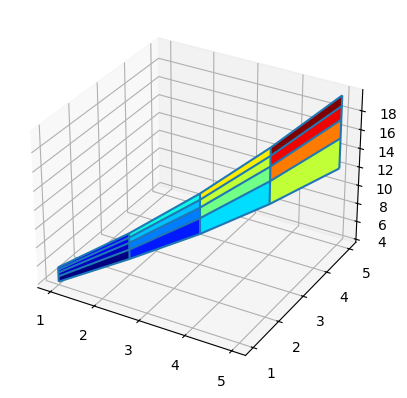
\includegraphics[width=0.5\textwidth]{media/inj_term_size_plane.png}
    \caption{3D projection of log term size of inj($M$) against $n,m$. There is an exponential relationship in both directions, creating a curved plane. A colour spectrum is used to highlight that the plane is curved in two directions, whereas redder colours indicate a larger term size.}
    \label{fig:3d-plane-term-size}
\end{figure}

\begin{figure}
\centering
\begin{subfigure}{0.45\textwidth}
  \centering
  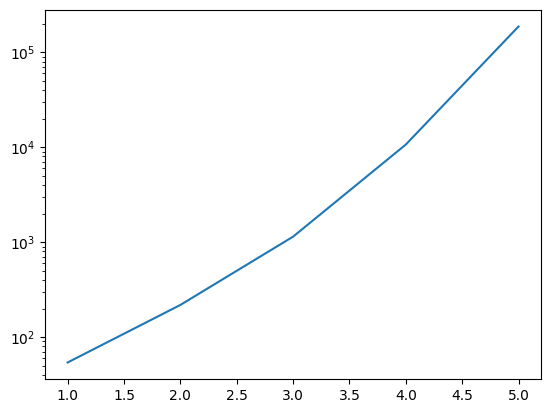
\includegraphics[width=\textwidth]{media/inj_term_size_against_type_order.png}
  \caption{Term size against the number of function parameters, where $n=1$ is fixed}
\end{subfigure}%
\hfill
\begin{subfigure}{0.45\textwidth}
  \centering
  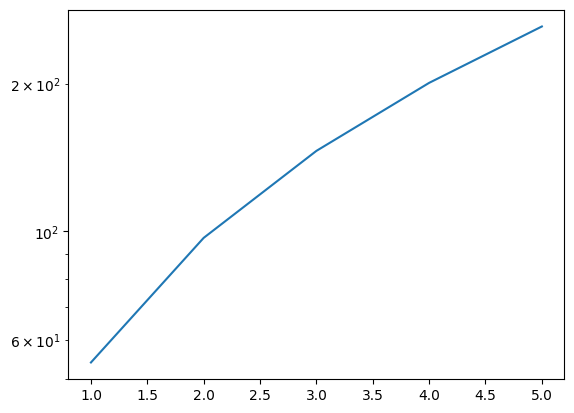
\includegraphics[width=\textwidth]{media/inj_term_size_against_upper_bound.png}
  \caption{Term size against the upper bound, where $m=0$ is fixed}
\end{subfigure}
\caption{Term size of inj($M$)in relation to hyperparameters $n,m$. Note the log scale. Together these act as slices of the 3D plane in Figure \ref{fig:3d-plane-term-size}}.
\label{fig:inj-term-size}
\end{figure}

\begin{figure}
\centering
\begin{subfigure}{0.45\textwidth}
  \centering
  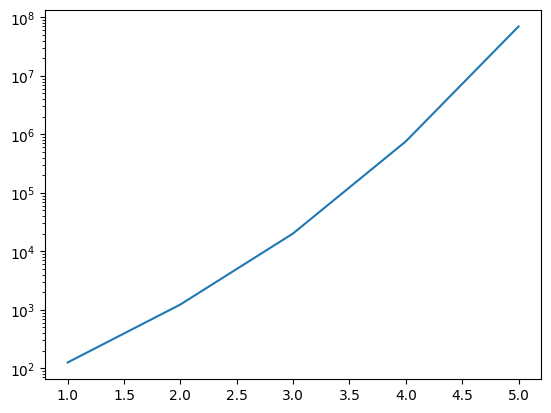
\includegraphics[width=\textwidth]{media/affine_term_size_against_type_order.png}
  \caption{Log term size against the number of function parameters, where $n=1$ is fixed}
\end{subfigure}%
\hfill
\begin{subfigure}{0.45\textwidth}
  \centering
  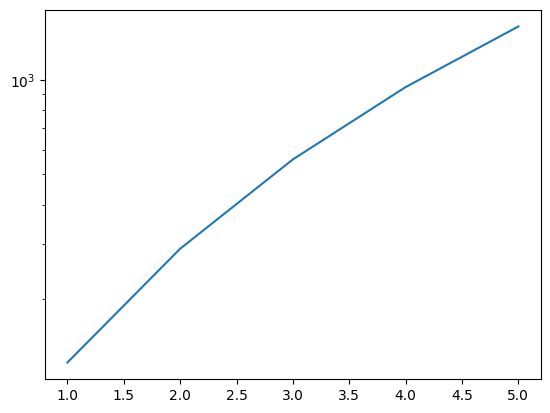
\includegraphics[width=\textwidth]{media/affine_term_size_against_upper_bound.png}
  \caption{Term size against the upper bound, where $m=0$ is fixed}
\end{subfigure}
\caption{Log term size of proj(inj($M$)) in relation to hyperparameters $n,m$.}
\label{fig:affine-term-size}
\end{figure}

\chapter{Example term transformation}

\begin{lstlisting}[mathescape, caption={Interpreter logs from applying injection and projection terms. The upper bound on values n = 2, effectively representing the booleans.}]
f = \p:(NatxNat) => Case <Case <1, p>, <$\bot$, $\bot$>>

proj(inj(f)) = 
\b:(NatxNat) => 
  Case <
    $\pi$1(Case <Catch (\p:(NatxNat) => Case <Case <1, p>, <$\bot$, $\bot$>>), 
        <<0, <(\a:Nat => Case <Case <1, <0, (Case <0, a>)>>, <$\bot$, $\bot$>>), (\a:Nat => Case <Case <1, <1, (Case <0, a>)>>, <$\bot$, $\bot$>>)>>,
        <1, <(\a:Nat => Case <Case <1, <(Case <0, a>), 0>>, <$\bot$, $\bot$>>), (\a:Nat => Case <Case <1, <(Case <0, a>), 1>>, <$\bot$, $\bot$>>)>>>>
      ),
    <(Case <Case <0, b>,
      <((Case <0, $\pi$2(Case <Catch (\p:(NatxNat) => Case <Case <1, p>, <$\bot$, $\bot$>>), 
          <<0, <(\a:Nat => Case <Case <1, <0, (Case <0, a>)>>, <$\bot$, $\bot$>>), (\a:Nat => Case <Case <1, <1, (Case <0, a>)>>, <$\bot$, $\bot$>>)>>, 
          <1, <(\a:Nat => Case <Case <1, <(Case <0, a>), 0>>, <$\bot$, $\bot$>>), (\a:Nat => Case <Case <1, <(Case <0, a>), 1>>, <$\bot$, $\bot$>>)>>>>)>
        ) <(Case <1, b>)>
        ), 
        ((Case <1, $\pi$2(Case <Catch (\p:(NatxNat) => Case <Case <1, p>, <$\bot$, $\bot$>>),
          <<0, <(\a:Nat => Case <Case <1, <0, (Case <0, a>)>>, <$\bot$, $\bot$>>), (\a:Nat => Case <Case <1, <1, (Case <0, a>)>>, <$\bot$, $\bot$>>)>>,
          <1, <(\a:Nat => Case <Case <1, <(Case <0, a>), 0>>, <$\bot$, $\bot$>>), (\a:Nat => Case <Case <1, <(Case <0, a>), 1>>, <$\bot$, $\bot$>>)>>>>)>
        ) <(Case <1, b>)>
        )>>
    ),
    (Case <Case <1, b>,
      <((Case <0, $\pi$2(Case <Catch (\p:(NatxNat) => Case <Case <1, p>, <$\bot$, $\bot$>>),
          <<0, <(\a:Nat => Case <Case <1, <0, (Case <0, a>)>>, <$\bot$, $\bot$>>), (\a:Nat => Case <Case <1, <1, (Case <0, a>)>>, <$\bot$, $\bot$>>)>>,
          <1, <(\a:Nat => Case <Case <1, <(Case <0, a>), 0>>, <$\bot$, $\bot$>>), (\a:Nat => Case <Case <1, <(Case <0, a>), 1>>, <$\bot$, $\bot$>>)>>>>)>
        ) <(Case <0, b>)>
        ),
        ((Case <1, $\pi$2(Case <Catch (\p:(NatxNat) => Case <Case <1, p>, <$\bot$, $\bot$>>),
          <<0, <(\a:Nat => Case <Case <1, <0, (Case <0, a>)>>, <$\bot$, $\bot$>>), (\a:Nat => Case <Case <1, <1, (Case <0, a>)>>, <$\bot$, $\bot$>>)>>,
          <1, <(\a:Nat => Case <Case <1, <(Case <0, a>), 0>>, <$\bot$, $\bot$>>), (\a:Nat => Case <Case <1, <(Case <0, a>), 1>>, <$\bot$, $\bot$>>)>>>>)>
        ) <(Case <0, b>)>
        )>>
    )>>

\end{lstlisting}

\chapter{Example program execution}\label{appendix: term evaluations}
\section{Program Definition}
\captionof{listing}{A program to find the factorial of a number in our implementation of SPCF.\label{listing:example-program-appendix}}
\begin{minted}[breaklines]{haskell}
addLeftTerm = \f:Nat->Nat->Nat => \x:Nat => \y:Nat => if0 x then y else (succ (f (pred x) y));
add = \x:Nat => \y:Nat => (fix addLeftTerm) x y;

mulTerm = \f:Nat->Nat->Nat => 
          \x:Nat => 
          \y:Nat => 
            if0 y 
              then x 
              else (add x (f x (pred y)));

mul = \x: Nat => \y:Nat => (fix mulTerm) x (pred y);

factorial = \f: Nat->Nat => \n:Nat => if0 n then 1 else (mul n (f (pred n)));
fact = \n: Nat => (fix factorial) n;

eval (fact 3);

\end{minted}

\section{Program Type Judgements}
\captionof{listing}{Interpreter logs for typing the program in \ref{listing:example-program-appendix}}
\begin{minted}[breaklines]{haskell}
Type judgement for addLeftTerm = \f:o->o->o => \x:o => \y:o => if0 x then y else (succ (f (pred x) y))
[f]: o->o->o
[x]: o
[y]: o
[pred x]: o
[f (pred x)]: o->o
[f (pred x) y]: o
[succ (f (pred x) y)]: o
[if0 x then y else (succ (f (pred x) y))]: o
[\y:o => if0 x then y else (succ (f (pred x) y))]: o->o
[\x:o => \y:o => if0 x then y else (succ (f (pred x) y))]: o->o->o
[\f:o->o->o => \x:o => \y:o => if0 x then y else (succ (f (pred x) y))]: (o->o->o)->o->o->o

Type judgement for add = \x:o => \y:o => (fix addLeftTerm) x y
[x]: o
[y]: o
[fix addLeftTerm]: o->o->o
[(fix addLeftTerm) x]: o->o
[(fix addLeftTerm) x y]: o
[\y:o => (fix addLeftTerm) x y]: o->o
[\x:o => \y:o => (fix addLeftTerm) x y]: o->o->o

Type judgement for mulTerm = \f:o->o->o => \x:o => \y:o => if0 y then x else add x (f x (pred y))
[f]: o->o->o
[x]: o
[y]: o
[pred y]: o
[f x]: o->o
[f x (pred y)]: o
[add x]: o->o
[add x (f x (pred y))]: o
[if0 y then x else add x (f x (pred y))]: o
[\y:o => if0 y then x else add x (f x (pred y))]: o->o
[\x:o => \y:o => if0 y then x else add x (f x (pred y))]: o->o->o
[\f:o->o->o => \x:o => \y:o => if0 y then x else add x (f x (pred y))]: (o->o->o)->o->o->o

Type judgement for mul = \x:o => \y:o => (fix mulTerm) x (pred y)
[x]: o
[y]: o
[pred y]: o
[fix mulTerm]: o->o->o
[(fix mulTerm) x]: o->o
[(fix mulTerm) x (pred y)]: o
[\y:o => (fix mulTerm) x (pred y)]: o->o
[\x:o => \y:o => (fix mulTerm) x (pred y)]: o->o->o

Type judgement for factorial = \f:o->o => \n:o => if0 n then 1 else mul n (f (pred n))
[f]: o->o
[n]: o
[1]: o
[pred n]: o
[f (pred n)]: o
[mul n]: o->o
[mul n (f (pred n))]: o
[if0 n then 1 else mul n (f (pred n))]: o
[\n:o => if0 n then 1 else mul n (f (pred n))]: o->o
[\f:o->o => \n:o => if0 n then 1 else mul n (f (pred n))]: (o->o)->o->o

Type judgement for fact = \n:o => (fix factorial) n
[n]: o
[fix factorial]: o->o
[(fix factorial) n]: o
[\n:o => (fix factorial) n]: o->o

Type judgement for eval {fact 3}
[3]: o
[fact 3]: o
[Evaluation] -- fact 3
\end{minted}

\section{Program Evaluation}
\captionof{listing}{Interpreter logs for the evaluation of the factorial of 3 \ref{listing:example-program-appendix}}
\begin{minted}[breaklines]{haskell}
Evaluating fact with environement:
("factorial",\f:o->o => \n:o => if0 n then 1 else mul n (f (pred n)))
+--("addLeftTerm",\f:o->o->o => \x:o => \y:o => if0 x then y else (succ (f (pred x) y)))
|  +--("add",\x:o => \y:o => (fix addLeftTerm) x y)
|  +--("fact",\n:o => (fix factorial) n)
+--("mul",\x:o => \y:o => (fix mulTerm) x (pred y))
   +--|
   +--("mulTerm",\f:o->o->o => \x:o => \y:o => if0 y then x else add x (f x (pred y)))

Apply (\n:o => (fix factorial) n) [3/"n"] 

Evaluating factorial with environement:
("factorial",\f:o->o => \n:o => if0 n then 1 else mul n (f (pred n)))
+--("addLeftTerm",\f:o->o->o => \x:o => \y:o => if0 x then y else (succ (f (pred x) y)))
|  +--("add",\x:o => \y:o => (fix addLeftTerm) x y)
|  +--("fact",\n:o => (fix factorial) n)
+--("mulTerm",\f:o->o->o => \x:o => \y:o => if0 y then x else add x (f x (pred y)))
   +--("mul",\x:o => \y:o => (fix mulTerm) x (pred y))
   +--("n",3)

Apply (\a:o => if0 a then 1 else mul a ((fix (\f:o->o => \n:o => if0 n then 1 else mul n (f (pred n)))) (pred a))) [3/"a"] 
if 3
 then 1
 else mul 3 ((fix (\b:o->o => \c:o => if0 c then 1 else mul c (b (pred c)))) (pred 3))

Finding predecessor of 3
Apply (\a:o => if0 a then 1 else mul a ((fix (\b:o->o => \c:o => if0 c then 1 else mul c (b (pred c)))) (pred a))) [2/"a"] 
if 2
 then 1
 else mul 2 ((fix (\d:o->o => \b:o => if0 b then 1 else mul b (d (pred b)))) (pred 2))

Finding predecessor of 2
Apply (\a:o => if0 a then 1 else mul a ((fix (\d:o->o => \b:o => if0 b then 1 else mul b (d (pred b)))) (pred a))) [1/"a"] 
if 1
 then 1
 else mul 1 ((fix (\c:o->o => \d:o => if0 d then 1 else mul d (c (pred d)))) (pred 1))

Finding predecessor of 1
Apply (\a:o => if0 a then 1 else mul a ((fix (\c:o->o => \d:o => if0 d then 1 else mul d (c (pred d)))) (pred a))) [0/"a"] 
if 0
 then 1
 else mul 0 ((fix (\b:o->o => \c:o => if0 c then 1 else mul c (b (pred c)))) (pred 0))

Evaluating mul with environement:
("factorial",\f:o->o => \n:o => if0 n then 1 else mul n (f (pred n)))
+--("addLeftTerm",\f:o->o->o => \x:o => \y:o => if0 x then y else (succ (f (pred x) y)))
|  +--("add",\x:o => \y:o => (fix addLeftTerm) x y)
|  |  +--("a",1)
|  |  +--|
|  +--("fact",\n:o => (fix factorial) n)
+--("mulTerm",\f:o->o->o => \x:o => \y:o => if0 y then x else add x (f x (pred y)))
   +--("mul",\x:o => \y:o => (fix mulTerm) x (pred y))
   +--("n",3)

Apply (\x:o => \y:o => (fix mulTerm) x (pred y)) [1/"x"] 
Apply (\a:o => (fix mulTerm) 1 (pred a)) [1/"a"] 

Finding predecessor of 1

Evaluating mulTerm with environement:
("factorial",\f:o->o => \n:o => if0 n then 1 else mul n (f (pred n)))
+--("addLeftTerm",\f:o->o->o => \x:o => \y:o => if0 x then y else (succ (f (pred x) y)))
|  +--("add",\x:o => \y:o => (fix addLeftTerm) x y)
|  |  +--("a",1)
|  |  +--|
|  +--("fact",\n:o => (fix factorial) n)
+--("mulTerm",\f:o->o->o => \x:o => \y:o => if0 y then x else add x (f x (pred y)))
   +--("mul",\x:o => \y:o => (fix mulTerm) x (pred y))
   +--("n",3)

Apply (\a:o => \b:o => if0 b then a else add a ((fix (\f:o->o->o => \x:o => \y:o => if0 y then x else add x (f x (pred y)))) a (pred b))) [1/"a"] 
Apply (\c:o => if0 c then 1 else add 1 ((fix (\b:o->o->o => \c:o => \d:o => if0 d then c else add c (b c (pred d)))) 1 (pred c))) [0/"c"] 
if 0
 then 1
 else add 1 ((fix (\a:o->o->o => \c:o => \d:o => if0 d then c else add c (a c (pred d)))) 1 (pred 0))

Evaluating mul with environement:
("factorial",\f:o->o => \n:o => if0 n then 1 else mul n (f (pred n)))
+--("addLeftTerm",\f:o->o->o => \x:o => \y:o => if0 x then y else (succ (f (pred x) y)))
|  +--("add",\x:o => \y:o => (fix addLeftTerm) x y)
|  |  +--("a",2)
|  |  +--|
|  +--("fact",\n:o => (fix factorial) n)
+--("mulTerm",\f:o->o->o => \x:o => \y:o => if0 y then x else add x (f x (pred y)))
   +--("mul",\x:o => \y:o => (fix mulTerm) x (pred y))
   +--("n",3)

Apply (\x:o => \y:o => (fix mulTerm) x (pred y)) [2/"x"] 
Apply (\a:o => (fix mulTerm) 2 (pred a)) [1/"a"] 

Finding predecessor of 1

Evaluating mulTerm with environement:
("factorial",\f:o->o => \n:o => if0 n then 1 else mul n (f (pred n)))
+--("addLeftTerm",\f:o->o->o => \x:o => \y:o => if0 x then y else (succ (f (pred x) y)))
|  +--("add",\x:o => \y:o => (fix addLeftTerm) x y)
|  |  +--("a",1)
|  |  +--|
|  +--("fact",\n:o => (fix factorial) n)
+--("mulTerm",\f:o->o->o => \x:o => \y:o => if0 y then x else add x (f x (pred y)))
   +--("mul",\x:o => \y:o => (fix mulTerm) x (pred y))
   +--("n",3)

Apply (\a:o => \b:o => if0 b then a else add a ((fix (\f:o->o->o => \x:o => \y:o => if0 y then x else add x (f x (pred y)))) a (pred b))) [2/"a"] 
Apply (\c:o => if0 c then 2 else add 2 ((fix (\b:o->o->o => \c:o => \d:o => if0 d then c else add c (b c (pred d)))) 2 (pred c))) [0/"c"] 
if 0
 then 2
 else add 2 ((fix (\a:o->o->o => \c:o => \d:o => if0 d then c else add c (a c (pred d)))) 2 (pred 0))

Evaluating mul with environement:
("factorial",\f:o->o => \n:o => if0 n then 1 else mul n (f (pred n)))
+--("addLeftTerm",\f:o->o->o => \x:o => \y:o => if0 x then y else (succ (f (pred x) y)))
|  +--("add",\x:o => \y:o => (fix addLeftTerm) x y)
|  |  +--("a",3)
|  |  +--|
|  +--("fact",\n:o => (fix factorial) n)
+--("mulTerm",\f:o->o->o => \x:o => \y:o => if0 y then x else add x (f x (pred y)))
   +--("mul",\x:o => \y:o => (fix mulTerm) x (pred y))
   +--("n",3)

Apply (\x:o => \y:o => (fix mulTerm) x (pred y)) [3/"x"] 
Apply (\a:o => (fix mulTerm) 3 (pred a)) [2/"a"] 

Finding predecessor of 2

Evaluating mulTerm with environement:
("factorial",\f:o->o => \n:o => if0 n then 1 else mul n (f (pred n)))
+--("addLeftTerm",\f:o->o->o => \x:o => \y:o => if0 x then y else (succ (f (pred x) y)))
|  +--("add",\x:o => \y:o => (fix addLeftTerm) x y)
|  |  +--("a",2)
|  |  +--|
|  +--("fact",\n:o => (fix factorial) n)
+--("mulTerm",\f:o->o->o => \x:o => \y:o => if0 y then x else add x (f x (pred y)))
   +--("mul",\x:o => \y:o => (fix mulTerm) x (pred y))
   +--("n",3)

Apply (\a:o => \b:o => if0 b then a else add a ((fix (\f:o->o->o => \x:o => \y:o => if0 y then x else add x (f x (pred y)))) a (pred b))) [3/"a"] 
Apply (\c:o => if0 c then 3 else add 3 ((fix (\b:o->o->o => \c:o => \d:o => if0 d then c else add c (b c (pred d)))) 3 (pred c))) [1/"c"] 
if 1
 then 3
 else add 3 ((fix (\a:o->o->o => \c:o => \d:o => if0 d then c else add c (a c (pred d)))) 3 (pred 1))

Finding predecessor of 1
Apply (\b:o => \e:o => if0 e then b else add b ((fix (\a:o->o->o => \c:o => \d:o => if0 d then c else add c (a c (pred d)))) b (pred e))) [3/"b"] 
Apply (\f:o => if0 f then 3 else add 3 ((fix (\e:o->o->o => \a:o => \c:o => if0 c then a else add a (e a (pred c)))) 3 (pred f))) [0/"f"] 
if 0
 then 3
 else add 3 ((fix (\b:o->o->o => \d:o => \a:o => if0 a then d else add d (b d (pred a)))) 3 (pred 0))

Evaluating add with environement:
("factorial",\f:o->o => \n:o => if0 n then 1 else mul n (f (pred n)))
+--("addLeftTerm",\f:o->o->o => \x:o => \y:o => if0 x then y else (succ (f (pred x) y)))
|  +--("add",\x:o => \y:o => (fix addLeftTerm) x y)
|  |  +--("a",2)
|  |  +--|
|  +--("fact",\n:o => (fix factorial) n)
|     +--("c",1)
|     +--|
+--("mulTerm",\f:o->o->o => \x:o => \y:o => if0 y then x else add x (f x (pred y)))
   +--("mul",\x:o => \y:o => (fix mulTerm) x (pred y))
   +--("n",3)

Apply (\x:o => \y:o => (fix addLeftTerm) x y) [3/"x"] 
Apply (\a:o => (fix addLeftTerm) 3 a) [3/"a"] 

Evaluating addLeftTerm with environement:
("factorial",\f:o->o => \n:o => if0 n then 1 else mul n (f (pred n)))
+--("addLeftTerm",\f:o->o->o => \x:o => \y:o => if0 x then y else (succ (f (pred x) y)))
|  +--("add",\x:o => \y:o => (fix addLeftTerm) x y)
|  |  +--("a",3)
|  |  +--|
|  +--("fact",\n:o => (fix factorial) n)
|     +--("c",1)
|     +--|
+--("mulTerm",\f:o->o->o => \x:o => \y:o => if0 y then x else add x (f x (pred y)))
   +--("mul",\x:o => \y:o => (fix mulTerm) x (pred y))
   +--("n",3)

Apply (\a:o => \b:o => if0 a then b else (succ ((fix (\f:o->o->o => \x:o => \y:o => if0 x then y else (succ (f (pred x) y)))) (pred a) b))) [3/"a"] 
Apply (\c:o => if0 3 then c else (succ ((fix (\b:o->o->o => \c:o => \d:o => if0 c then d else (succ (b (pred c) d)))) (pred 3) c))) [3/"c"] 
if 3
 then 3
 else succ ((fix (\a:o->o->o => \c:o => \d:o => if0 c then d else (succ (a (pred c) d)))) (pred 3) 3)

Finding successor of (fix (\a:o->o->o => \c:o => \d:o => if0 c then d else (succ (a (pred c) d)))) (pred 3) 3

Finding predecessor of 3
Apply (\b:o => \e:o => if0 b then e else (succ ((fix (\a:o->o->o => \c:o => \d:o => if0 c then d else (succ (a (pred c) d)))) (pred b) e))) [2/"b"] 
Apply (\f:o => if0 2 then f else (succ ((fix (\e:o->o->o => \a:o => \c:o => if0 a then c else (succ (e (pred a) c)))) (pred 2) f))) [3/"f"] 
if 2
 then 3
 else succ ((fix (\b:o->o->o => \d:o => \a:o => if0 d then a else (succ (b (pred d) a)))) (pred 2) 3)

Finding successor of (fix (\b:o->o->o => \d:o => \a:o => if0 d then a else (succ (b (pred d) a)))) (pred 2) 3

Finding predecessor of 2
Apply (\c:o => \e:o => if0 c then e else (succ ((fix (\b:o->o->o => \d:o => \a:o => if0 d then a else (succ (b (pred d) a)))) (pred c) e))) [1/"c"] 
Apply (\f:o => if0 1 then f else (succ ((fix (\e:o->o->o => \b:o => \d:o => if0 b then d else (succ (e (pred b) d)))) (pred 1) f))) [3/"f"] 
if 1
 then 3
 else succ ((fix (\a:o->o->o => \c:o => \b:o => if0 c then b else (succ (a (pred c) b)))) (pred 1) 3)

Finding successor of (fix (\a:o->o->o => \c:o => \b:o => if0 c then b else (succ (a (pred c) b)))) (pred 1) 3

Finding predecessor of 1
Apply (\d:o => \e:o => if0 d then e else (succ ((fix (\a:o->o->o => \c:o => \b:o => if0 c then b else (succ (a (pred c) b)))) (pred d) e))) [0/"d"] 
Apply (\f:o => if0 0 then f else (succ ((fix (\e:o->o->o => \a:o => \c:o => if0 a then c else (succ (e (pred a) c)))) (pred 0) f))) [3/"f"] 
if 0
 then 3
 else succ ((fix (\b:o->o->o => \d:o => \a:o => if0 d then a else (succ (b (pred d) a)))) (pred 0) 3)
"6"
\end{minted}
\end{document}
